\pdfoutput=1

\documentclass{4thYearProject}

\makeatletter\@openrightfalse\makeatother
\usepackage{graphicx}
\usepackage{tabularx}
\usepackage{diagbox}
\usepackage{hyperref}
\usepackage{float}
\usepackage{longtable}
\usepackage{listings}
\usepackage{color}
\usepackage{pdfpages}

% Used for subsubsections %
\usepackage{titlesec}
\setcounter{secnumdepth}{4}
\setcounter{tocdepth}{4}

% Checkmark %
\usepackage{amssymb}

\definecolor{dkgreen}{rgb}{0,0.6,0}
\definecolor{gray}{rgb}{0.5,0.5,0.5}
\definecolor{mauve}{rgb}{0.58,0,0.82}

\newcolumntype{Y}{>{\raggedleft\arraybackslash}X}

\graphicspath{ {resources/images/} }

\begin{document}
\title{A Microissue Approach to Project Management}
\author{Alex Leet}
\date{2016/2017}
\maketitle

\begin{abstract}
Issue, or ticket, oriented project management is emerging as the defacto standard in the software industry.  Project tasks (feature implementation, bug fixes) are encapsulated in self-contained records, called tickets.  A variety of tools exist to support this method, which brings the ability to keep track of tasks in collaborative, distributed teams. However,  research in Software Engineering has identified that ticket records are not always maintained with all the information pertinent to the resolution of an issue.  It is hypothesised that one reason for this problem is the need for a software developer to context switch between completing the main task in a development environment and the user interface for a ticket management system in order to maintain a ticket.  The project proposes the concept of microissues to investigate how tickets which reside in source code could be an alternative means of project management. A prototype plugin was built for IntelliJ IDEA in order to demonstrate the concept and from the user evaluation and background research done, it was discovered that in certain cases it could indeed be a viable method of issue management.

\end{abstract}

\pagebreak
\renewcommand{\abstractname}{Acknowledgements}
\begin{abstract}

I would like to thank Dr. Timothy Storer for the supervision of the project, facilitating the requirements gathering process and providing valuable ideas for a smooth continuation of the project on a weekly basis. Additional thanks go to all the volunteers who agreed to take part in the user evaluation.

\end{abstract}
\educationalconsent

\tableofcontents
%==============================================================================

\chapter{Introduction}
\pagenumbering{arabic}

\section{Motivation \& Context}

Issue management holds an important part in the process of software development. Numerous issue management systems to aid issue tracking exist, however, the majority are either client-server applications, distributed or hosted systems. Based on the research described in section \ref{sec:Research} and the already existing plugins, there is a lack of attempts to reduce context switch between using issue management systems and computer programming. The importance of doing so is to improve productivity and provide a less strenuous way for developers to convey important information relating to the project worked on.

\section{Objectives}

The prime objective of the project is to develop a working plugin prototype with minimal features that demonstrate the concept of how a source code issue management system could work, which will then be used for user evaluation including gathering feedback to gain an understanding of users' perspective on how it compares to traditional issue tracking. Research on existing plugins relating to issue management should be done to draw a conclusion of similar attempts made so far and existing research on issue management should be analysed in order to evaluate the exact aspects of issue management that hold the most importance for developers in software development. 

\section{Achievements}

The plugin developed conforms to the initial idea and encapsulates an issue management system based on tickets residing in source code. Background research was made on similar plugins, which allowed to gain an overview of similar attempts made so far, with important lessons learned in terms of display of issues in such plugins. Prior research was analysed and it has certified the importance of documentation that requires little effort, which code-level documentation is a prime candidate of. Additionally, user evaluation was performed to assess the working of the plugin and a survey was then conducted on usability and informal opinion on how the users felt the plugin compared to the issue tracking systems they have previously used. The results showed that there is a highly positive feedback in regards to the likelihood of usage of the plugin, especially in regards to personal projects. This in combination with the results of prior research demonstrates that the concept of microissues could be a viable software management tool.

\section{Dissertation Structure}

The structure of the dissertation is delineated as follows. Chapter 2 presents the background relating to the project, including an overview of related plugins and existing research done on issue management. Chapter 3 reviews the functional and non-functional requirements gathered, providing a description and justification of each. In addition, the software process decisions are outlined. Chapters 4 details the final design of the plugin, presenting various parts of the plugin. Chapter 5 details the implementation of the plugin, including the alternatives considered and the justifications for the final decisions taken. Chapter 6 discusses the means performed in order to evaluate the plugin, which were unit testing and user evaluation. Chapter 7 presents the conclusion of the dissertation and discusses the outcome of the project, future work possibilities, the learning outcomes and an overall summarisation. 


\chapter{Background}

This chapter discusses the specifics of issue tracking systems and outlines related work - in particular the already existing plugins relating to issue tracking and also discusses research on how developers perceive issue tracking and what part it plays in their software development process.

\section{Issue Tracking}

Issue tracking is the process of documenting and keeping track of tasks or defects that occur during development. It is considered a vital part of software development process and can be considered as a means of communication within the development team \cite{socialnature}. 

An issue tracking system is a computer software that is used create and track the aforementioned issues. They essentially act as databases that store all the relevant information pertaining the status updates on issues from their creation to completion \cite{socialnature}. 

In issue tracking systems the electronic artefacts representing a particular task, bug, epic or story are commonly known as issues or tickets. They contain various information with the most common fields being:

\begin{itemize}
\item \textbf{Summary} - The summarisation of the purpose of the ticket.
\item \textbf{Type} - The type of the ticket, most commonly either a task, bug, user story or an epic. 
\item \textbf{Status} - At which stage the completion of the ticket is in.
\item \textbf{Priority} - The importance of the ticket compared to other tickets.
\item \textbf{Resolution} - Why the ticket was set as completed.
\item \textbf{Assignee} - Who is responsible for completion of the ticket.
\item \textbf{Estimated time} - How long the completion of the ticket is estimated to take.
\end{itemize}

In addition to the above mentioned, the available fields of entry can vary from one system to another and in some, custom creation of fields according to a team's needs is possible. 

\section{Related Work}

Various plugins have been developed to ease the integration of issue management and integrated development environments (IDEs). However, as the below mentioned examples will demonstrate, most are intended to connect to the various issue management systems available. 

\subsection{Inbuilt IntelliJ Task Management Plugin}

IntelliJ IDEA is bundled with its own task management plugin and is activated by default \cite{intellijtaskplugin}. It allows for integration to various issue tracking systems, which provides the user with the functionality to open, create and delete tasks or issues as shown in Figure \ref{fig:intellijtask}. In addition, users can create local tasks, however, they are not visible to other users and are not archived in any way. An additional interesting feature of the inbuilt plugin is the ability to create context, which is tying a set of files in the editor to a particular task. When the user decides to work on a different task, the files in the editor are changed to the files tied to that task. This allows the developer to focus on the relevant sections of the code.   

\begin{figure}[H]
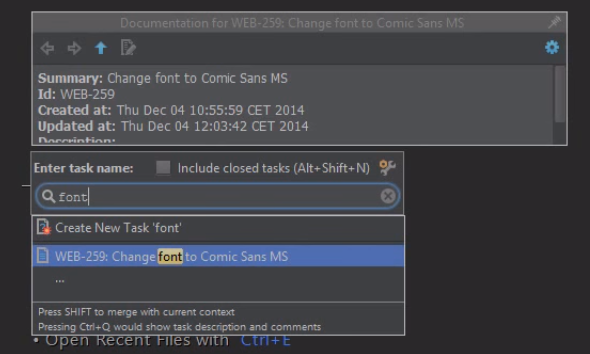
\includegraphics[scale=0.5]{IntelliJ_Tasks}
\centering
\caption{Example of viewing a YouTrack task in IntelliJ.}
\label{fig:intellijtask}
\end{figure}

\subsection{Tasks Navigation Plugin}

An attempt to connect source code to issue management systems in order to reduce context switch was made by Vladislav Rassokhin, who developed the plugin \textit{Tasks Navigation} \cite{tasksnavigation} that allows the user to link to issues in the Web from comments and reference injections in IntelliJ as shown in Figure \ref{fig:tasksnavigation}. With the plugin it is easy to quickly get information about the issue by clicking on the relevant link in the comment and since the comment resides close to the code in question, it is easy to see which part of code the issue particularly pertains to. 

\begin{figure}[H]
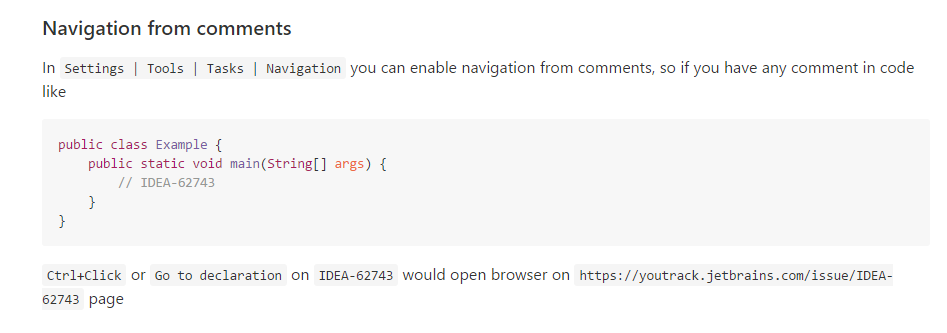
\includegraphics[scale=0.6]{Tasks_Navigation_Plugin}
\centering
\caption{Example of how the Tasks Navigation plugin works}
\label{fig:tasksnavigation}
\end{figure}

\subsection{Tasks Plugin}

Tasks\cite{tasksplugin} is an IntelliJ plugin allowing users to locally create and manage tasks and issues. The plugin was deemed highly relevant to the project due to its well-structured interface and a wide array of features as demonstrated in Figure \ref{fig:tasks}. In addition to the basic capability of creating, modifying and deleting issues, the plugin also includes the ability to assign priorities to tasks, filter them by priorities and keep track for how long they have been worked on. However, there is no possibility to connect the tasks to source code in order to see the relevant code relating to the task. 

\begin{figure}[H]
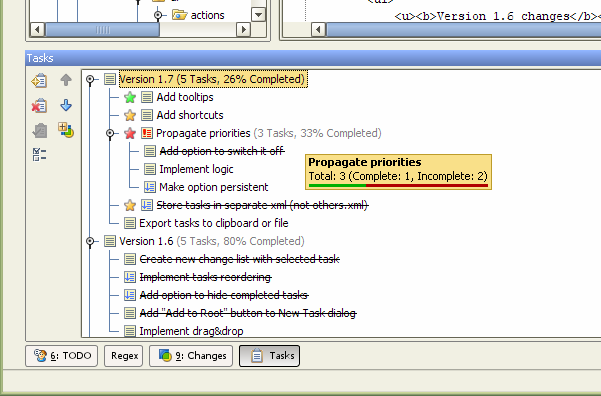
\includegraphics[scale=0.6]{Tasks}
\centering
\caption{Example of task management in the Tasks plugin.}
\label{fig:tasks}
\end{figure}

\subsection{Mylyn}

Mylyn is the task and application lifecycle management (ALM) framework for Eclipse \cite{mylyn}. It boasts a wide array of features, including being able to work on either local tasks, which do not require a shared repository, or shared repository tasks, which do. Similarly to the IntelliJ's built in plugin it allows to create certain views around tasks, which allows to specify the exact files that have to be worked on for the specific task. A sample view of tickets in Mylyn can be seen in Figure \ref{fig:mylyn}.

\begin{figure}[H]
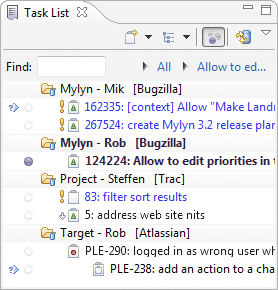
\includegraphics[scale=0.7]{Mylyn}
\centering
\caption{Example view of tasks in Mylyn in Eclipse.}
\label{fig:mylyn}
\end{figure}

\subsection{Eclipse TODO Editor Plugin}

The Eclipse todo editor plugin allows to edit todo files in Eclipse \cite{todoeditor}, which are then displayed in a panel. This plugin deserves a mentioned due to the fact that it allows users to readily view all the tasks (todos) that they have defined in a nicely formatted tree in Eclipse itself (as shown in Figure \ref{fig:eclipsetodo} and therefore allows them for a more focused approach to what has to be achieved. 

\begin{figure}[H]
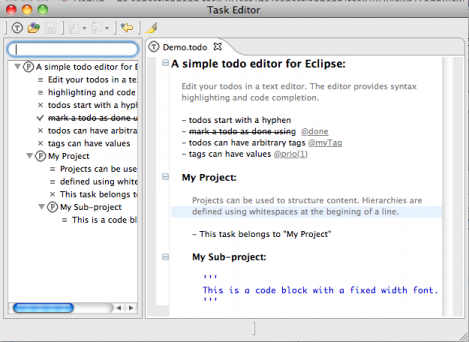
\includegraphics[scale=0.6]{eclipse_TODO_editor}
\centering
\caption{Example of the editor window, including the visual display of todo's on the left.}\label{eclipsetodo}
\label{fig:eclipsetodo}
\end{figure}

\subsection{Summary of Related Work}

All of the above mentioned plugins were developed with a specific purpose in mind. However, they can be mainly divided into two categories:

\begin{itemize}
\item Plugins intended to be used with an already existing issue management system available. 
\item Plugins that act as standalone issue management systems themselves.
\end{itemize}

A summarisation of the plugin features can be viewed in the table \ref{table:featurematrix}.

\begin{center}
\begin{table}[H]
\noindent
\begin{tabular}{|l|*{5}{c|}}\hline
\backslashbox[50mm]{Plugin}{Feature}
&\makebox{Integration with source code}&\makebox{Local issue management}&\makebox{Display of all issues}
\\\hline
IntelliJ Inbuilt Plugin & Partial & \checkmark & \checkmark \\\hline
Tasks Navigation & \checkmark &  & \\\hline
Tasks &  & \checkmark & \checkmark \\\hline
Mylyn & Partial  & \checkmark & \checkmark \\\hline
Eclipse TODO Editor &  & \checkmark & \checkmark \\\hline
\end{tabular}
\caption{Feature matrix of related plugins}
\label{table:featurematrix}
\end{table}
\end{center}

From the summarisation of the features it can be observed that a lot of the plugins researched do not connect tickets to source code in almost any way. The only exception is the \textit{Tasks Navigation} plugin, however, since it only provides the ability to link to external issue management systems, it does not allow for ticket creation or modification within the IDE itself.

It can also be observed that the display of all issues is a prominent feature and in all cases, issues are displayed to the user as a list. This fact is an inspiration for the design of the plugin.

\section{Research on Issue Tracking and Usage of Issue-tracking Systems}\label{sec:Research}

Attempts have been made to research recording of issues and bugs and the common shortcomings of how bugs and issues are documented. A study by Jorge Aranda and Gina Venolia has found that one of the most crucial bits of information missing in issue management is links to source code and the change-sets that resolved these bugs \cite{lifeofbugs}. Additionally, they had found that in some cases, the key events in the story of a bug had left no electronic trace and therefore there was no way to discover the important information pertaining the fixing of a bug.

One of the interview results in the research paper "How Software Engineers Use Documentation: The State of the Practices" is that software engineers value documentation that requires little effort but still serve as important historical information and such code-level comments are one of the most preferred methods of documentation since they are short and rest within the source code, therefore resulting in very little maintenance work  \cite{stateofpractice}. 

The importance of being able to readily view information from the development environment is also strengthened by the existence of documentation tools such as JavaDoc and Doxygen, which both provide a rich set of useful information at low effort \cite{usingjavadoc}.

\section{Summary of Related Work and Research}

The related plugins and existing research on issue tracking display that there have definitely been attempts to optimise software development process by finding means of conveying important information as efficiently as possible. The related plugins demonstrate the prevalence of a list-based view of issues in the IDE for easier view of tasks to work and concentrate on. The issue management plugins that are shipped with the Eclipse and IntelliJ IDEA Java IDEs both feature the ability to create certain views and tie tasks to particular files to be worked on, which further proves the importance of focused software development. The research on issue tracking and usage on issue tracking systems outlines the importance of electronic trace of tasks and bugs of the project and that documentation that lies with the source code is of high value to developers, which could also be considered the motivation behind documentation tools.

\chapter{Requirements}

This chapter discusses the process of requirements gathering performed and presents the attained requirements of the project, including functional, non-functional and software process requirements. 

\section{Requirements Elicitation and Gathering}

Project requirements were gathered and discussed throughout weekly meetings with Dr. Timothy Storer of Computing Science department at the University of Glasgow. Both functional and non-functional requirements had to be carefully considered due to the fact that the aim of the project was a working prototype of the plugin with enough minimal features that would allow to gather feedback on the concept of microissues and how it compares to standard issue management. 

%https://ocw.mit.edu/courses/aeronautics-and-astronautics/16-885j-aircraft-systems-engineering-fall-2005/readings/sefguide_01_01.pdf%

\section{Functional Requirements}

Functional requirements define what the system must be able to do and are defined as features of the system \cite{systemfundamentals}. Of the following functional requirements, in order to demonstrate the concept of microissues, the definite requirements of utmost importance were related to the basic functionality of an issue management system - creating and modifying tickets. The complete list of functional requirements gathered is as follows.

\subsection{Allow the User to Create Tickets}

In order for the plugin to function as a local issue management system, the ability for the user to create tickets is a key feature to be included. 

Due to the nature of the project, the tickets have to explicitly reside in the source code and therefore a way for the user to explicitly signify a ticket without impacting the rest of the code has to be considered. Such a ticket is the very definition of a microissue.

\subsection{Detect User Created Tickets}

The created tickets should be detected by the plugin, either as they are being created or after the user has finished creating the ticket. 

\subsection{Allow the User to Delete Tickets}

The user should be able to delete their created tickets and the plugin should reflect the fact that they were deleted. 

\subsection{Allow the User to Modify a Ticket}

The user should be able to modify the created ticket and the changes made should be reflected when viewing a ticket's information.

\subsection{Display the Tickets}

The detected tickets should be displayed in order for the user to get an overview of all the issues created.

\subsection{Display Ticket Information}

Ticket information has to be displayed when a particular ticket is selected and must include all the relevant information that the user has specified when creating the ticket.

\subsection{View a Ticket's History}

Ticket's history throughout version control commits has to be retrieved with the appropriate changes indicated, including the information relating to the commit itself - the date and the committer details.

\subsection{Sort Tickets and Filter Tickets}

In order for the developer to focus on specific tasks in particular, the ability to filter and sort tasks should be implemented. For example, the user should be able to sort tickets either by their type or priority. 

\section{Non-Functional Requirements}

Non-functional requirements describe what qualities the system should have and their primary objective is to ensure the satisfaction with the system \cite{nonfunctional} and that the plugin does not impact the rest of the IDE.

\subsection{Usability}

The creation and management of tickets should be simple, quick and not require expert knowledge. The user should be able to get help on how to use the plugin relatively quickly.

\subsection{Performance}

The plugin should not impact the overall performance of the IDE. The ticket creation, detection and display should therefore be relatively fast in order to match the performance of other features of the IDE in order not to disrupt the workflow of the developer. 

\subsection{Reliability}

The plugin should not be prone to crashes and exceptions. In the case crashes do occur, they should not prevent the user from using any other features of the IDE apart from the ones relating to the plugin.  

%http://www.bredemeyer.com/pdf_files/NonFunctReq.PDF%

\section{Software Process Requirements}

As the plugin was to be developed for the IntelliJ IDEA Java IDE, the obvious development language was to be Java. No specific requirements were placed on the version control software and an issue tracking system. Due to familiarity and ease of use, Git \cite{git} was chosen as the version control system with GitHub \cite{github} as the project hosting service, where the project was stored \cite{repo}. YouTrack \cite{youtrack}, a browser-based issue tracking system developed by JetBrains, was chosen as the issue management system for the project \cite{youtracklink}, which was used to store tasks to be completed, which were mostly defined after the weekly project meetings. 

\chapter{Design}

This chapter presents the final design of the plugin, including an overview of all the design components. 

The design of the plugin followed iterative development cycles and follows a similar style of the other features in the IDE as shown in Figure \ref{fig:fulldesign}. Each individual design component is described and demonstrated in the following sections.

\begin{figure}[H]
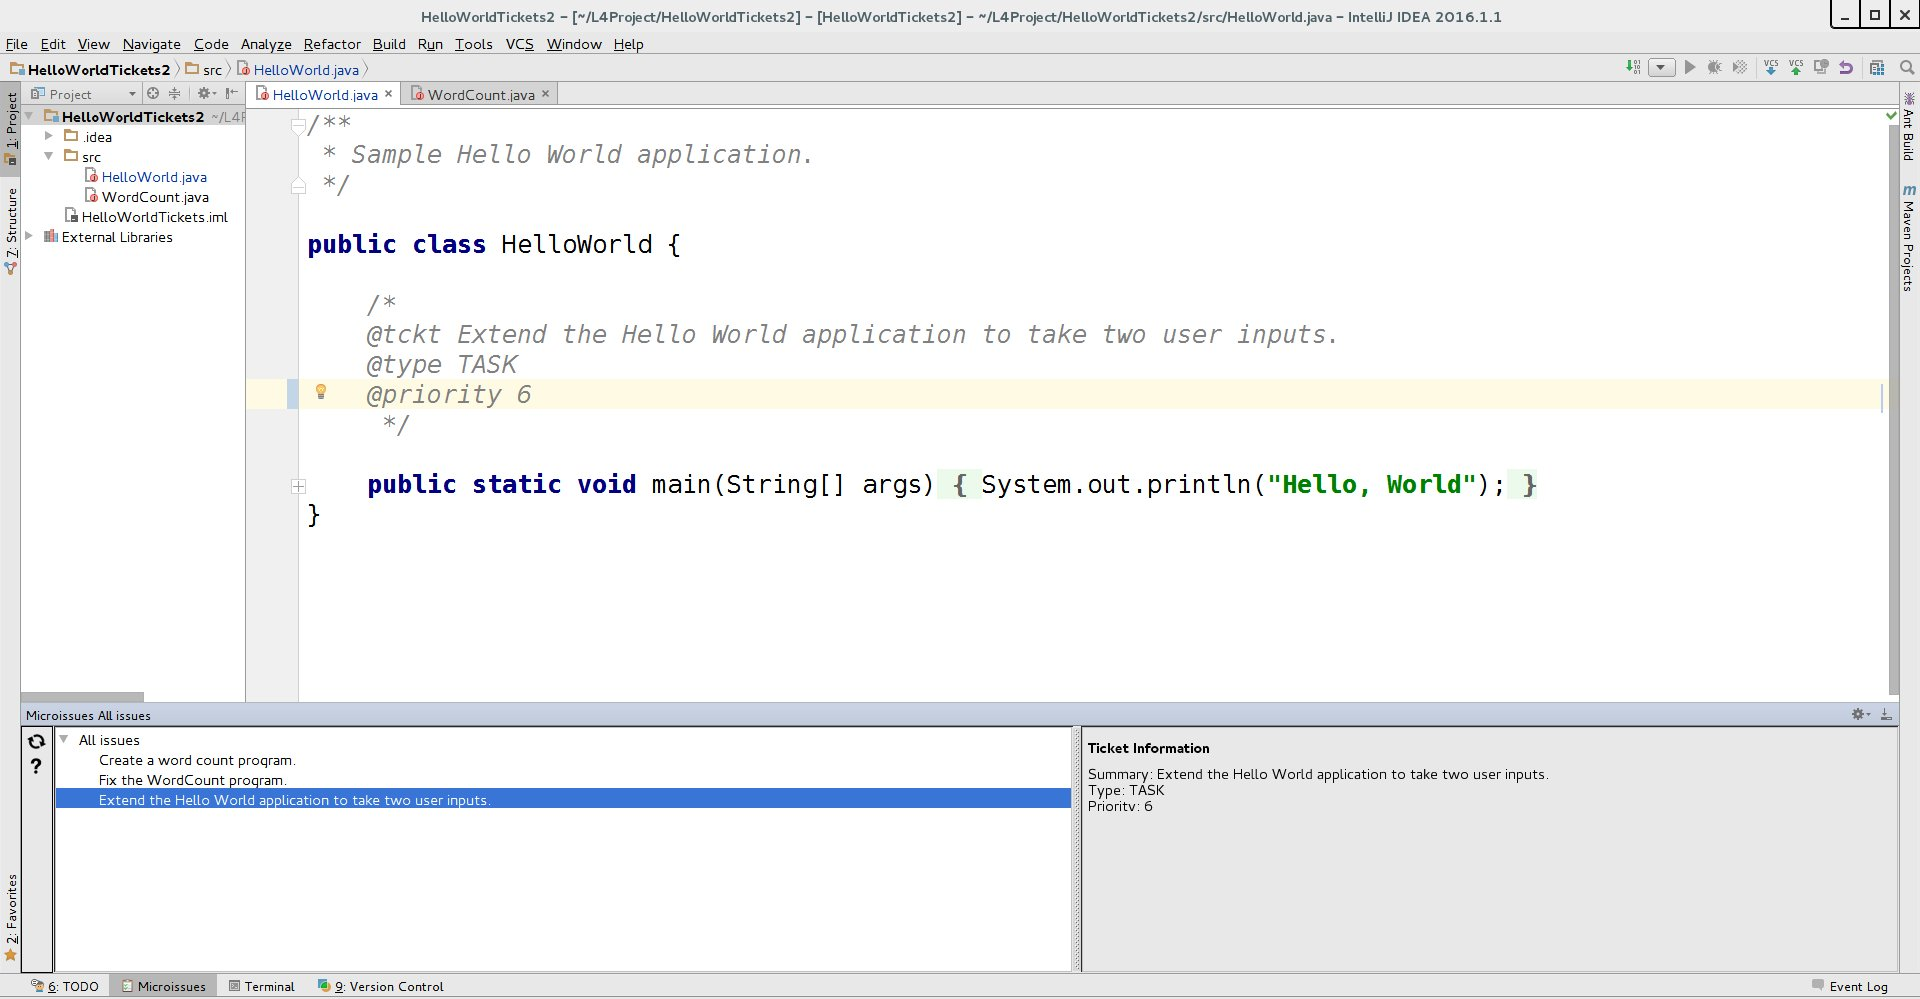
\includegraphics[scale=0.35]{Full_design_white}
\centering
\caption{The final design of the plugin displaying all the relevant components.}
\label{fig:fulldesign}
\end{figure}

\section{Main Tool Window}

The plugin features an openable tool window anchored to the bottom of the IDE and is the main mean of displaying information to the user. The tool window is separated into the following components: 

\begin{itemize}
\item Toolbar for helper commands
\item Ticket tree display
\item Ticket information display
\end{itemize}

\subsection{Toolbar}\label{sec:toolbar}

The toolbar is responsible for providing helper commands, which are visualised as clickable icons, to the user. \newline
From top to bottom the commands are:
\begin{itemize}
\item Display help dialog
\item Refresh all the tickets
\end{itemize}

\begin{figure}[H]

\includegraphics[scale=0.6]{Toolbar_figure_white}
\centering
\caption{The toolbar with the helper command icons: refresh (top), help dialog (bottom).}\label{toolbar}
\label{fig:toolbar}
\end{figure}

% Figure here %
\subsubsection{Help dialog}

The help dialog presents the user the information on what the plugin does and how ticket creation works. 

\begin{figure}[H]
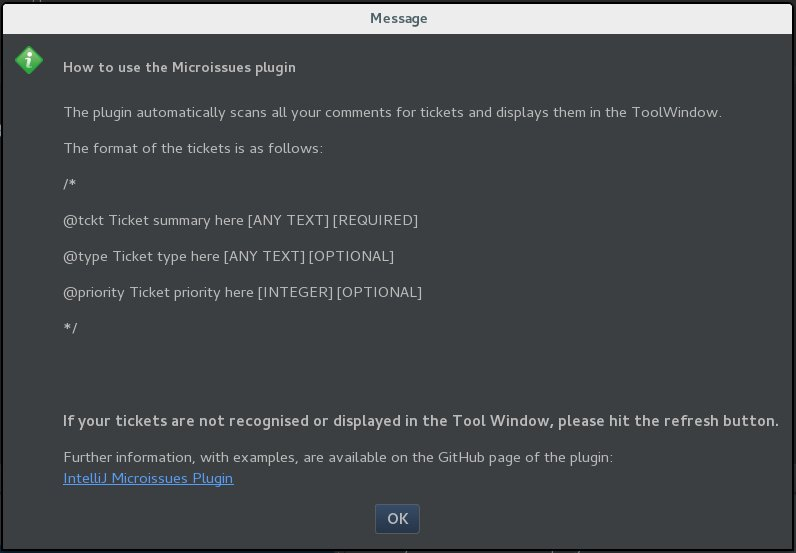
\includegraphics[scale=0.6]{HelpDialog}
\centering
\caption{The displayed help dialog after the user clicks on the icon}\label{helpdialog}
\label{fig:helpdialog}
\end{figure}

% Figure here %

\subsubsection{Refresh command}

The refresh command refreshes all the tickets in the case that there are discrepancies between the tickets they have typed and the tickets that are displayed in the ticket tree.

\subsection{Ticket Tree Panel}

The ticket tree panel contains a scrollable pane that contains a tree of all the tickets. Each of the nodes correspond to either:
\begin{itemize}
\item Ticket summary, if the ticket is a ticket in the current version of the source code. 
\item Change details and commit date if the ticket is an older version of the ticket rec. 
\end{itemize}

The design of both can be seen in Figure \ref{fig:tasktree}, with the tickets "Create a word count program", "Fix the WordCount program" and "Extend the Hello World Application to take two user inputs" representing the current tickets in the source code, while the "Multiple Changes: Committed on Thu Feb 16 13:13:27 GMT 2017" representing an older version of the "Extend the Hello World application to take two user inputs" ticket, indicating that there have been multiple changes to the ticket and when the commit was made. 

\begin{figure}[H]
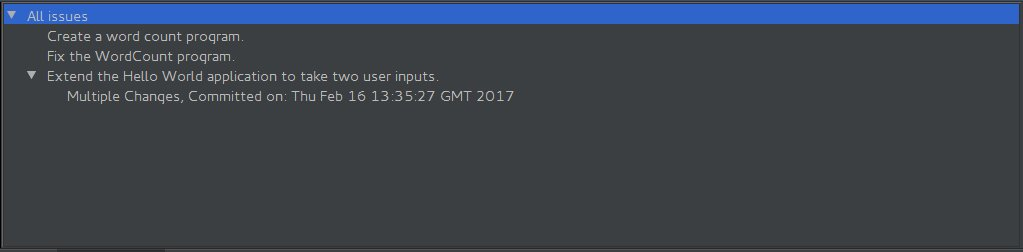
\includegraphics[scale=0.6]{Task_tree_all}
\centering
\caption{The panel containing the tree view of tickets, including regular tickets and an older ticket version.}
\label{fig:tasktree}
\end{figure}

\subsection{Ticket Information Panel}

The ticket information panel displays information about the ticket. Similarly to the ticket tree, there is a distinction between the information displayed for a current ticket and an older ticket. The distinction is as such:

\begin{itemize}
\item Current ticket - Ticket information is displayed for all the available information of the ticket, which can be seen in Figure \ref{fig:ticketpanel}.

\begin{figure}[H]
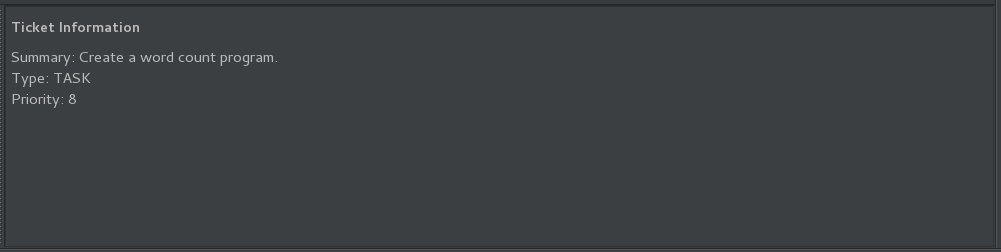
\includegraphics[scale=0.6]{Ticket_infopanel}
\centering
\caption{The panel displaying ticket information.}\label{ticketpanel}
\label{fig:ticketpanel}
\end{figure}

\item Old ticket - In addition to the above details, the old ticket additionally has the commit information (the date and the committer) and which fields are different (as shown in Figure \ref{fig:oldticketpanel}).
\end{itemize}

\begin{figure}[H]
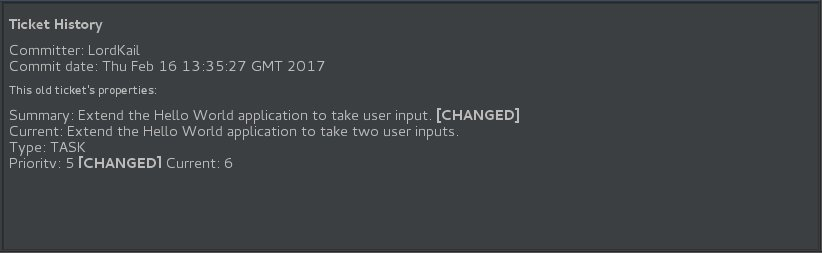
\includegraphics[scale=0.7]{OldTicket_infopanelV2}
\centering
\caption{The panel displaying an older ticket's information.}\label{oldticketpanel}
\label{fig:oldticketpanel}
\end{figure}

\section{Retrieving Ticket History}

The ticket history is retrieved by right clicking a ticket in the task tree, which brings up a pop-up dialog as demonstrated in Figure \ref{fig:popup}.

\begin{figure}[H]
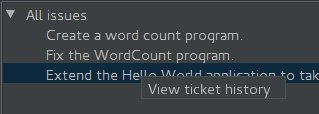
\includegraphics[scale=0.7]{View_history}
\centering
\caption{The pop-up dialog prompted on right click with the option to view ticket history.}
\label{fig:popup}
\end{figure}

Clicking on the pop-up dialog brings up a message prompting the user to select the root folder of their application, where the .git folder is stored as shown in Figure \ref{fig:selectfolder}.

\begin{figure}[H]
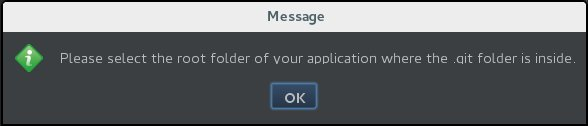
\includegraphics[scale=0.7]{Folder_select_message}
\centering
\caption{The message prompting the user to select the root folder of their application .}
\label{fig:selectfolder}
\end{figure}

Lastly, the user is presented with the actual file chooser dialog where they have to navigate to the folder as shown in Figure \ref{fig:filechooser} and pressing \textit{Open} initiates the retrieval of the older tickets (if they exist) and are presented to the user as previously shown in Figure \ref{fig:tasktree}.

\begin{figure}[H]
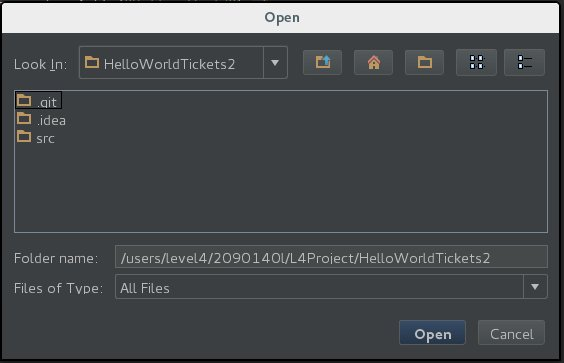
\includegraphics[scale=0.7]{File_chooser}
\centering
\caption{The file chooser dialog, demonstrating an example folder that the user would have to navigate to.}
\label{fig:filechooser}
\end{figure}

\chapter{Architecture}

This chapter discusses the architecture of the plugin and outlines the implementation details of its functionality.

The development process for most of the components of the plugin was iterative, with some features requiring a redesign due to the shortcomings in prior implementation techniques that were discovered throughout development. 

The architecture of the plugin will be outlined and discussed in the following sections in the natural order that the plugin operates in. 

\section{Plugin startup}

The initial concern was considering how and when the plugin should be started. Two different approaches were tried:
\begin{itemize}
\item Implementing the \textit{ProjectComponent} interface  
\item Implementin the \textit{StartupActivity} interface 
\end{itemize}

\subsection{ProjectComponent}

The project component is a component, which is associated to a plugin. The implementation class, in this project's case \textit{ToolWindowComponent.java}, becomes a component, which can be accessed from anywhere in the code using the \textit{getComponent(class)} method on an instance of a Project. In order for the implementation to be recognised as a component, it has to be registered in the \textit{plugin.xml} as such:\\

\begin{lstlisting}[language=XML, 
basicstyle={\scriptsize\ttfamily}, 
frame=single,
showstringspaces=false,
breaklines=true,
,tabsize=3]
<project-components>
    <component>
      <implementation-class>uk.ac.glasgow.microissues.ui.ToolWindowComponent</implementation-class>
    </component>
</project-components>
\end{lstlisting}

Initially this approach was used to create the tool window and at the same time, start the process of scanning the files for comments. This approach worked until it was discovered that it threw an exception when the project took a slightly longer time to load. The exception thrown was that PSI elements could not be accessed while the project was loading and therefore a different approach had to be found. 

\subsection{StartupActivity}

The \textit{StartupActivity} interface allows the implementation class to be run after the project has initialized and loaded. This is done by registering it in the \textit{plugin.xml} as a \textit{postStartupActivity}:   \\

\begin{lstlisting}[language=XML, 
basicstyle={\scriptsize\ttfamily}, 
frame=single,
showstringspaces=false,
breaklines=true,
,tabsize=3]
<postStartupActivity implementation="uk.ac.glasgow.microissues.ui.SetupToolWindow"></postStartupActivity>
\end{lstlisting}

It was discovered, however, that this approach did not work for initialising the tool window as during some occurrences it would not appear. However, when it did, it was apparent that an exception when scanning the files for comments was not thrown and that led to the solution.

\subsection{Solution}

The importance of having discussed both of the approaches above is that the appropriate solution found was using a mixture of both of these techniques. 

The \textit{initComponent} and \textit{projectOpened} methods from the \textit{ProjectComponent} interface were used to initialize and register the tool window to the project as a component and using the \textit{runActivity} method from the \textit{StartupActivity} interface allowed to start the process of scanning the files for comments without an exception being thrown.

\section{UI Components}

The implementation of the plugin consists of several UI components to provide containers for the tickets and ticket information retrieved. IntelliJ IDEA uses Swing, which is a collection of Java GUI components, for its user interface and therefore all the UI components used for the plugin are Swing components and are as follows:\\ 
\newline
\textbf{ToolWindow}
\newline
The main tool window of the plugin contains a basic \textit{JPanel}, which is a container for grouping components together. In this case it is used to contain a \textit{JSplitPane}. \\
\newline
\textbf{JSplitPane}
\newline
The \textit{JSplitPane} is a container for dividing two separate components. The JSplitPane was used to separate the \textit{JBScrollPane} containing a \textit{JTree} that held all the tickets and a \textit{JBScrollPane} that held the \textit{JPanel} for displaying ticket information.
\newline\\
\textbf{JBScrollPane}
\newline
The \textit{JBScrollPane} is IntelliJ IDEA's extension of the Swing's \textit{JScrollPane}, which allows the content of the panel to be scrolled if the content is greater than the size of panel. This is used so that the panel containing the ticket tree can be scrolled when there are a lot of tickets or if the ticket information window contains too much information and has to be scrolled.\\
\newline
\\
\textbf{JTree}
\newline
The JTree is Java Swing's component for presenting hierarchical data and is used for displaying the tickets as a tree. When an object is added to the JTree as a node, the nodes shown in the tree use the object's \textit{toString} method to display the appropriate text.\\
\newline
\textbf{JPanel}
\newline
The JPanel is a lightweight container used for storing basic components - in this case a JPanel is used to store the JLabel to display text.  \\ 
\newline
\textbf{JLabel}
\newline
The JLabel is a display area for displaying text, images or both. It accepts HTML markup language , which allows for the text to be displayed in a flexible way using the HTML tags.\\ 
\newline
\textbf{JEditorPane}
\newline
JEditorPane is a component for display text and was used to display the help message presented the user. JEditorPane was used as the help message was to include a link to the github repository of the project for further information, however, the standard HTML way of creating a URL link does not work with regular JLabels. The JEditorPane allows to create a hyperlink by adding a HyperLinkListener to it, which will listen to the clicks on the specified hyperlink. 
\section{Tickets}

A ticket is represented in the code as a C-style comment with a particular structure. A user can signify a ticket by using the \textit{@tckt} annotation, followed by the sample summary that describes the ticket. \\
This particular tag is required if the user wishes to transform the comment into a ticket, with the rest of the tags optional. The exact tags allowed and the accepted entries are as follows:

\begin{itemize}
\item \textit{@tckt} - Has to be followed by a string, signifying the summary of the ticket.  
\item \textit{@type} - Signifies the type of the ticket. Has to be followed by any string.
\item \textit{@priority} - Signifies the importance of the ticket. Has to be followed by an integer.
\end{itemize}

The figure \ref{fig:ticketcomment} demonstrates  how a sample comment intended to be a ticket looks like.

\begin{figure}[H]
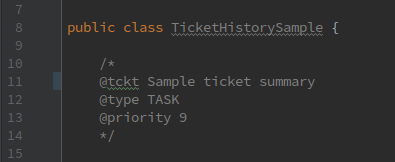
\includegraphics[scale=0.6]{Ticket_comment}
\centering
\caption{An example of a ticket represented as a comment in the code.}\label{ticketcomment}
\label{fig:ticketcomment}
\end{figure}

As tickets reside as comments in the code, a way to extract them and turn them into actual ticket instances was necessary. This was accomplished by utilising Program Structure Interface (PSI) elements, the collection of which represents an internal structure of the source code in the IntelliJ Platform. \\

To store data relating to a particular ticket, the \textit{Ticket} class was created.

\begin{figure}[H]
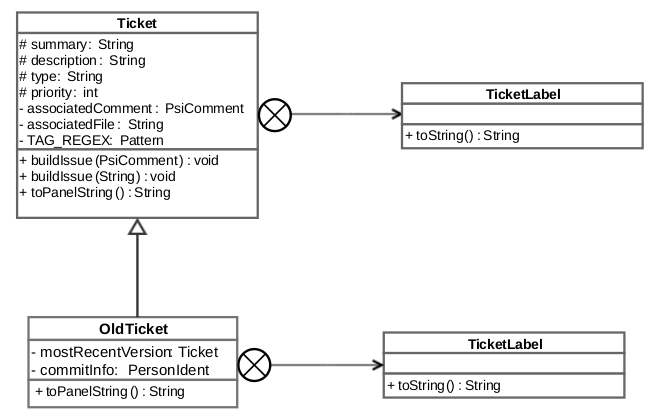
\includegraphics[scale=0.6]{Ticket_UML}
\centering
\caption{The UML diagram of the Ticket class presenting its inner class and the subclass.}
\label{fig:ticketuml}
\end{figure}

As shown in figure \ref{fig:ticketuml}, the Ticket class contains variables for all the important data relating to a ticket - the summary, type, description and the priority. The \textit{associatedComment} variable keeps track of the PSI element that contains the comment, which is the ticket, and the \textit{associatedFile} variable keeps track of the file that the comment resides in. The Ticket class is extended by the OldTicket class which is used for storing information about the older ticket versions. 

\subsection{TicketLabel}

The \textit{TicketLabel} inner classes of both \textit{Ticket} and \textit{OldTicket} are used solely for overriding the \textit{toString} method, which is used to display information in the task tree. For example, in the case of the \textit{Ticket} class, the \textit{TicketLabel} \textit{toString} method is represented as following:

\begin{lstlisting}[language=Java, basicstyle=\footnotesize\tt,        % the size of the fonts that are used for the code
  frame=single,                    % adds a frame around the code
  language=Java,                 % the language of the code
  keywordstyle=\bf]
@Override
public String toString(){
	return summary;
}
\end{lstlisting}

This means that when passing the \textit{TicketLabel} class to a Java JTree as a node will ensure that the ticket's summary will be displayed in the tree. 

The \textit{TicketLabel} inner class of the \textit{OldTicket} follows the same principle, however, the string returned is the concatenation of the following:

\begin{itemize}
\item An indication of what is different between the old ticket and the current ticket
\item The commit date displayed in Java's standard date format.
\end{itemize}  

\subsection{PSI Tree Traversal \& PSI Comments}

Comments are scanned and found by traversing the PSI tree of the whole project at the start of the plugin. IntelliJ treats comments as instances of \textit{PsiComment} which is a subclass of \textit{PsiElement}. 

The main purpose of PSI elements was to retrieve their type and text. The text of the PSI element is retrieved by calling the \textit{getText} method that would return the text that the PSI element represents. For example, the \textit{PsiComment} instance would return the full text of the comment if the \textit{getText} method was called on it. Using PSI elements and the PSI tree, the process of traversing the project and finding PSI comments is as follows.

\begin{enumerate}
\item All files in the project are found.
\item For each Java file in the project:
\begin{enumerate}
\item Get the PSI element representing that Java file.
\item Recursively go through each child of the PSI element and check whether it is an instance of a PSI comment.
\item If it is and the comment text contains the tag \textit{@tckt}, build the ticket.
\end{enumerate}
\end{enumerate}

The process of finding all the files in the project was done by using a \textit{ContentIterator}. This allowed to iterate through each file in the project, represented as a \textit{VirtualFile}, which is the IntelliJ Platform's way of representing files in a file system. 

\textit{VirtualFiles} allowed to retrieve the type of the file (in this case, Java files were the sought after files) and also the corresponding PSI element (an instance of \textit{PsiFile} - a PSI element representing a file) of that file, which would allow us to start recursively finding instances of PSI comments.  

\subsection{Ticket Building}

The ticket building is performed by calling the \textit{buildTicket} method on a \textit{Ticket} instance, with the PSI element specified as a parameter. 

The \textit{buildTicket} method extracts the text via the aforementioned \textit{getText method}, the corresponding filename the comment resides in and records the corresponding PSI element. A regular expression matching on the extracted text is then performed. \\
\newline
The exact regular expression pattern used in the code is:
\begin{lstlisting}[language=Java, basicstyle=\footnotesize\tt,        % the size of the fonts that are used for the code
  frame=single,                    % adds a frame around the code
  language=Java,                 % the language of the code
  keywordstyle=\bf]
 private static final Pattern TAG_REGEX = Pattern.compile("@(.+?)\\s(.+?)\\n");
\end{lstlisting}

This regular expression matches all lines that contain an @ with any string directly after it without any whitespaces and then a string separated by any whitespace delimiters. For example, a valid entry that this regular expression will match is \textit{@tckt Sample summary} in which it will capture the tag "@tckt" as the first capture group and the followed text "Sample summary" as the second capture group. However, this places certain limitations on the developer when creating tickets - mainly the fact that each of the ticket attributes have to be one line entries. Even though this is a limitation for the developer, it was chosen due to better reliability and greatly simplifies the process of creating tickets.

\section{PsiTreeChangeListener}

With tickets residing in source code, it is important to detect when a comment containing the ticket is added, removed, changed or moved, in order to represent the most current state of the tickets at all times. This removes the necessity for the user to explicitly signify when they have made a change.

The IntelliJ Platform Plugin Software Development Kit (SDK) does not provide a direct way to monitor a particular PSI element. Instead, it provides a \textit{PsiTreeChangeListener} interface that upon implementation listens for changes in the project's PSI tree and invokes the appropriate methods. The particular methods that were used are:

\begin{itemize}
\item public void childAdded(@NotNull PsiTreeChangeEvent event) - invoked when a PsiElement has been added.
\item public void childRemoved(@NotNull PsiTreeChangeEvent event) - invoked when a PsiElement has been removed.
\item public void childReplaced(@NotNull PsiTreeChangeEvent event) - invoked when a PsiElement has been changed.
\item public void childrenChanged(@NotNull PsiTreeChangeEvent event) - invoked when a lot of PsiElements have been changed at once.
\item public void propertyChanged(@NotNull PsiTreeChangeEvent event) - invoked when a PsiElement's property has changed.

\end{itemize}

\subsection{Initial approach}

The initial approach to using the \textit{PsiTreeChangeListener} was to create, delete and update tickets on individual basis based on the corresponding PSI element that was changed. \\
For example, if an already existing comment that contained a ticket was edited, the associated ticket would be rebuilt based on the newer version of the comment. This involved locating a ticket with the corresponding PSI element and calling the \textit{buildTicket} method on that ticket.  

It was discovered, however, that this approach was unstable due to the nature of the PSI elements changing in a very unpredictable and quick manner and often, complex nested statements had to be written in order to ensure that no exception would be thrown due to a lost reference to a PSI element. 

This became an even more serious issue when multiple tickets existed in the same file and the user tried to delete the first ticket character by character. If they deleted the trailing comment ending */, everything from the start of the leading /* of the first comment up to the ending */ of the second comment would be considered a comment. IntelliJ would instantaneously lose the reference to the PSI element that corresponded to the second ticket which caused the two following problems:

\begin{itemize}
\item An exception was thrown when the user tried to view the ticket information of the second ticket.
\item If the user restored the first comment, two duplicate tickets of the second ticket would exist in the task tree.
\end{itemize}

Based on these issues encountered and the difficulty of dealing with PSI elements on individual basis, an alternative approach had to be devised.

\subsection{Simplification}

Due to the shortcomings of the previous method, the code was restructured in order to handle changes to the PSI tree differently. \\
The new and currently used method involves associating tickets to the file they reside in. When a PSI element change is detected the following workflow occurs:

\begin{itemize}
\item The PSI element that triggered the PsiTreeChangeListener is checked whether it is a ticket and if so:
\begin{itemize}
\item Previous tickets in the task tree relating to the file that the PSI element is in are removed.
\item The file is rescanned for complete tickets and are displayed in the task tree. 
\end{itemize}
\end{itemize}

The following Java code demonstrates how this approach simplified the process:\\

\begin{lstlisting}[language=Java, basicstyle=\footnotesize\tt,        % the size of the fonts that are used for the code
  frame=single,                    % adds a frame around the code
  language=Java,                 % the language of the code
  keywordstyle=\bf]
  @Override
  public void childAdded(@NotNull PsiTreeChangeEvent event) {
  	elementAddedOrRemoved(event, event.getChild());
  }

  @Override
  public void childRemoved(@NotNull PsiTreeChangeEvent event) {
  	elementAddedOrRemoved(event, event.getChild());
  }

  @Override
  public void childReplaced(@NotNull PsiTreeChangeEvent event) {
  	elementAddedOrRemoved(event, event.getOldChild());
  	elementAddedOrRemoved(event, event.getNewChild());
  }

\end{lstlisting}

It can be observed that in the three different cases, whether the PSI element is added, removed or modified, the same method is called. The method \textit{elementAddedOrRemoved} is responsible for finding out which file the element is in and initiating a re-scan of tickets in that file. In contrast to the initial implementation, where the three methods were drastically different, this approach was proven to be significantly less prone to exceptions.  

\section{Ticket History}

Viewing ticket history There were mainly two options under consideration for recording and retrieving ticket history. The choice was to either associate a ticket with an ID or use approximate string matching. \\
\newline
\textbf{Associating a ticket with an ID} \\
\newline
When the user creates a ticket by writing the comment, an ID would either be generated automatically or they would add an ID themselves. When desired, the old ticket versions would then be retrieved from version control history by finding tickets with the same ID.
Even though this approach would provide accurate results in terms of finding older ticket versions, the problem is ensuring that the ID of the ticket is not compromised in any way after initial creation. For example, if a user created a ticket and it was assigned an ID and then the user changed the ticket ID by accident, it would signify a different ticket or possibly cause issues with the plugin. Due to the foreseeable issues with sustainability of the IDs, this idea was rejected. 
\\
\newline
\textbf{Approximate String Matching}\\
\newline
Approximate string matching is a technique for evaluating how similar two given strings are. This approach could be used to evaluate how similar a ticket and an older ticket are and if they are similar enough, the older ticket could be considered that ticket's older version. The similarity of the strings is measured as a percentage and various algorithms exist to retrieve it. 

This approach was chosen due to the fact that it is less likely to beak due to human error and at the same time, an assumption is made that if a ticket is too different to an older ticket, it is considered to be a completely separate ticket.  

The particular algorithm and implementation used was developed by the GitHub user msubhash \cite{fuzzywuzzy} and it uses Levenshtein Distance, which is considered to be one of the most important measures of similarity \cite{tourstringmatch}, to calculate the differences between sequences. 

For example, as presented by msubhash, the algorithm will return the following ratios for the following example string comparisons:

\begin{lstlisting}[language=Java, basicstyle=\footnotesize\tt,        % the size of the fonts that are used for the code
  frame=single,                    % adds a frame around the code
  language=Java,                 % the language of the code
  keywordstyle=\bf,
  showstringspaces=false]
"CSK vs RCB", "RCB vs CSK" -----------> 100% match

"web services as a software", "software as a services" -----------> 100% match

"software-as-a-service", "software as a service" -----------> 100% match

"Microsoft's deal with skype", "Microsoft skype deal" -----------> 100% match

"apple is good", "Google is best apple is" -----------> 62% match

\end{lstlisting}

In order for the algorithm to be properly used in the plugin, particular ratios had to be decided on in order to consider an older ticket a ticket's previous version. Upon experimentations, 70\% was considered a reasonable ratio above which (but not 100\% as that would imply exactly the same ticket) the assumption would be made. 

\subsection{JGit}

The ability to view ticket history was developed by using the JGit Java library \cite{jgit}. It allows to access git commit history and retrieve various information pertaining a commit, such as:

\begin{itemize}
\item Diffs between files of the commit, each represented as a \textit{DiffEntry} instance.
\item Committer identity (username, email).
\item Commit date.
\end{itemize}

\subsection{Old Tickets}

The old tickets represent the previous versions of the ticket. In addition to the regular ticket, they carry information about the commit they were found in. They also include overridden methods for displaying the information in a different way in the task tree and the information panel. 

\section{Helper Classes}

The helper classes are registered as actions in \textit{plugin.xml} that get executed when the appropriate icon is clicked.

The following markup signifies the two helper classes, \textit{RefreshTasks.java} and \textit{HelpDisplayer.java} as actions with a corresponding icon:

\begin{lstlisting}[language=XML, 
basicstyle={\scriptsize\ttfamily}, 
frame=single,
showstringspaces=false,
breaklines=true,
,tabsize=3]
<action id="Refresh_tasks" class="uk.ac.glasgow.microissues.actions.RefreshTasks" icon="/uk/ac/glasgow/microissues/icons/refresh.png"></action>

<action id="DisplayHelpDialog" class="uk.ac.glasgow.microissues.actions.HelpDisplayer" text="Display help dialog" description="Displays the help dialog to inform the user how to use the plugin" icon="/uk/ac/glasgow/microissues/icons/help.png"></action>

\end{lstlisting}

These actions are then registered to the toolbar (as visualised in \ref{sec:toolbar}). %SOmething here some description?

\begin{lstlisting}[language=XML, 
basicstyle={\scriptsize\ttfamily}, 
frame=single,
showstringspaces=false,
breaklines=true,
,tabsize=3]
<group id="TasksAdditionalToolBarGroup" class="com.intellij.openapi.actionSystem.DefaultActionGroup">
      <reference ref="Refresh_tasks"/>
      <reference ref="DisplayHelpDialog" />
</group>

\end{lstlisting}


The \textit{RefreshTasks} class performs the same functionality that is performed when the plugin is started - all the existing tickets are deleted from the tree and the Java files of the project are scanned for tickets. 

The \textit{HelpDisplayer} class contains a \textit{JEditorPane} that is used to display a message formatted with HTML to the user.

\chapter{Evaluation}

The purpose of evaluation was to ascertain the quality of the final product and to gather feedback on the conceptual idea of the plugin and its purpose. The methods for evaluating the plugin were unit testing, for which metrics were gathered, and user evaluation, for which qualitative and quantitative data was gathered.

\section{Unit Testing}

% Describe what Unit Testing is 
In order to ensure that the critical sections of the logic in the final product to be deployed worked as intended, unit testing was incorporated. Unit testing was chosen due to the fact that it provides a quick way to verify   The following libraries were used:

\begin{itemize}
\item JUnit - the framework for writing unit tests widely used in Java.
\item EasyMock - the framework allowing to mock objects in order to simulate their behavior and values their methods return. 
\item Objenesis - a java library allowing to instantiate objects of particular class that have constructors with multiple arguments. Used by EasyMock in order to mock such objects.
\end{itemize}

From gathering the test coverage from running the tests, only 35\% of all classes are covered with a total 26\% line coverage. However, this is mostly due to the fact that a significant part of the plugin was either based on UI components or involved using anonymous classes as listeners. Unit testing is not viable for the scope. However, a major part of the plugin package, which contained the main code for building tickets and displaying ticket information was tested with the code coverage shown in Figure \ref{fig:codecoveragelines}.
 
\begin{figure}[H]
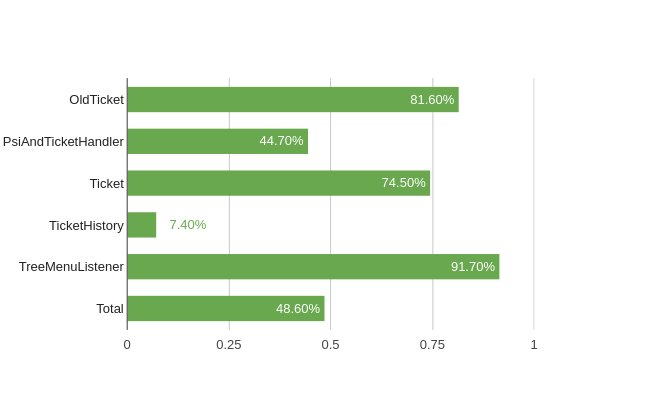
\includegraphics[scale=0.7]{code_coverage_lines}
\centering
\caption{Code coverage of lines of the plugin package .}
\label{fig:codecoveragelines}
\end{figure}

This ensures and verifies that the main functionalities of the plugin work as intended and return the expected results.  

\section{User evaluation}\label{sec:usereval}

Initially, user evaluation was intended to be carried out in a single iteration with all the users using the exact same deployed plugin. However, due to unexpected issues in the plugin that were discovered by the first few users, the evaluation had to be split into two iterations. 

\subsection{Preparation for Evaluation}

In order to evaluate the plugin, the following prerequisites had to be completed:

\begin{enumerate}
\item Deploy the plugin - the plugin was built and archived as a zip file containing all the necessary dependencies and the plugin itself so that the plugin can be tested on the users' machines to confirm portability. 
\item Create a sample project with existing tickets - necessary for the users to see sample tickets already created in order to hasten the familiarisation with the plugin.
\end{enumerate}


\subsection{General Structure of User Evaluation}

In both iterations 1 and 2, the structure and the flow of the evaluation was the same:

\begin{enumerate}
\item Confirm the users' consent and reassure anonymity.
\item Present the context of the project and general overview of the plugin.
\item Install the plugin for the IntelliJ IDE on their computer.
\item Present the user with the tasks to complete.
\item Gather feedback by providing them a survey link.
\end{enumerate}

Likewise, the tasks presented to the users remained the same and are according to the following script:

\begin{table}[H]
\centering
\def\arraystretch{1.5}
\begin{tabular}{p{5cm}p{10cm}}
\hline
Task & Description\\
\hline
1. View a ticket's information. & The user should be able to view all the relevant information pertaining the ticket in the information panel. \\
2. Edit an existing ticket. & The user should make changes to an existing ticket and ensure their changes are reflected in the task tree \& information panel. \\
3. Create a new ticket. & The user should create a new ticket by example of already existing tickets and ensure their ticket is visible in the task tree with the correct details in the information panel.  \\
4. Delete a ticket. & The user should delete the comment containing the ticket and ensure the ticket is gone from the task tree. \\
5. Move a ticket & The user should move a ticket (most likely cut-paste the comment to a different file or part of the code and ensure the ticket is not affected in the task tree or the information panel (no duplicates or removal of the ticket should occur).\\
6. View ticket history. & The should press to view the ticket history by right clicking the ticket in the task tree and the ticket history should \\ 
7. Experiment freely & The user is given the freedom to experiment with the plugin in any other way they could envisage it to be used. \\
\hline
\end{tabular}
\caption{Tasks for the user}
\label{table:userevaltasks}
\end{table}

\subsection{Iteration 1}

During the first iteration, the first version of the deployed plugin was used. A total of five users were used for the evaluation. As previously discussed, issues were discovered during the iteration which impacted some functionality of the plugin. \\
\newline
The issues discovered were as follows:\\
\newline
\textbf{Issue 1} - An exception thrown when creating or modifying a comment.\\
\newline
As soon as the user tried to create a comment in order to create the ticket, an exception would be thrown. If the user tried to make the comment a ticket by specifying the \textit{@tckt} tag, it would not be detected by the plugin and therefore not displayed in the task tree.\\   
\newline
\textbf{Cause \& Solution} - The issue was caused by the part of the code that was responsible for retrieving the filename of the file that the ticket would be associated to. The initial approach was to a call a single \textit{getParent()} method on the element and assume that it would be the element representing the class (including the name, which would be extracted). However, when a ticket is added inside nested parts of the code, the parent returned turned out to not be the class file but rather other elements in the hierarchy. Therefore the solution was to continuously go up in the hierarchy until the instance of the class file would be found.\\ 
\newline
\textbf{Issue 2} - An exception thrown when clicking an empty space in the task tree panel.\\
\newline
When the user tried to click on a ticket in the tree but missed and clicked an empty space, a \textit{ClassCastException} was thrown.\\
\newline
\textbf{Cause \& Solution} - when the mouse listener was added to the JTree containing the tasks, the assumption was that it would only detect clicks on the tree. However, that was not the case and clicks were registered everywhere in the panel and when clicking on a space that did not contain a ticket, instead of the \textit{Ticket} object retrieved, an empty string was returned instead. Therefore, when the clicked element was attempted to be casted as a \textit{Ticket}, the \textit{ClassCastException} would occur. The solution was to check after the click whether the retrieved object is a string and if so, no functionality would be executed. 

\subsection{Iteration 2}

The rest of the evaluation (12 users) was carried out in iteration 2. Issues found in iteration 1 were rectified as per the above solutions. During this iteration, none of the previously occurred issues emerged, however, a new issue was discovered by one of the users during their free exploration stage. \\
\newline
\textbf{Issue 1} - Tickets from Java files with identical names (in separate packages) are only detected from one of them.\\
\newline
A user had discovered this by creating two separate packages and creating Java files with identical names in them. It was observed that no tickets were displayed in the task tree, which was a serious concern although the reason was found by the means of debugging. \\
\newline
\textbf{Cause \& Solution} - The cause of the issue was the fact that since tickets were associated with the files they were in, when a scan of the file for tickets occurred, it would delete the previously detected tickets associated with that file from the task tree and re-add the new ones found. That meant if there were two files with the same name, only tickets from one of them would be displayed in the tree (and if one of the files was empty, if it was scanned last, none of the tickets from the first would be displayed).  Since this was an edge case and did not impact the overall working of the program, the iteration was continued with the deployed version. A solution was not deployed due to time constraints, however, a possible solution would be to tie tickets to files not only by the file name but also by the package namespace.

\subsection{Feedback Survey \& Evaluation results}

After the users had completed their tasks and free exploration of the plugin, they were provided a link to fill an optional survey in order to gather qualitative and quantitative feedback on the plugin and the concept of source code integrated issue tracking.\\
\newline
\textbf{How easy was the plugin to use?}\\
This question incorporated a linear scale of 1 to 5, with 1 being an indicator of an easy to use system that beginners (very little experience with the plugin) could use and 5 being an indicator of the opposite - a lot of experience and expert level knowledge of the plugin required for proper usage.   

\begin{figure}[H]
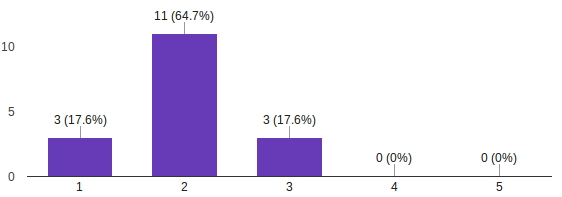
\includegraphics[scale=0.6]{How_easy}
\centering
\caption{Responses to how easy the plugin is to use.}
\label{fig:howeasy}
\end{figure}

Even though the question does not provide a benchmark of how easy the plugin is to use compared to other similar plugins or systems, it does provide feedback on how quickly the users can start using it and how accessible it is. Higher values would also indicate an increased confusion in users of what they can actually do. 
From the figure \ref{fig:howeasy} it can be seen that the highest volume of answers is in the lower spectrum. With the highest amount of answers being number 2, it indicates that the plugin required some getting used to and possibly looking at the plugin description window but was eventually easy to use with little learning curve. 

\textbf{Did you encounter any issues?}

This particular question was to ascertain the stability of the system and to record any unexpected issues that might have occurred during the completion. The checkbox options provided to the user were as follows:
% Is this list fine? %
\begin{itemize}
\item The plugin did not work as intended.
\item There were crashes/bugs.
\item Plugin installation did not work.
\item It was difficult to understand what the plugin is supposed to do.
\item It was hard to know what functionality the plugin allows.
\item None
\item Other (Textual entry)
\end{itemize}

Users encountered only the two of the above mentioned problems, which were that the plugin did not work as intended and that there were crashes and bugs. A total of 6 out of 17 users indicated this. The 5 responses were from the first iteration, which is due to the two issues discovered in that iteration and the sixth response was from the second iteration, where the issue with the filenames were discovered. Overall no correlation was found between facing issues and responses to the rest of the questions, which is most likely due to the fact that the users were ascertained of the fact that the plugin in question was a prototype intended to demonstrate a concept. 

\textbf{How do you feel this compares to standard issue management systems (Trac, GitLab, Jira)?}

The question featured a long textual entry box with the intention of receiving qualitative feedback on the plugin compared to the issue trackers that the users had previously used. Both user groups (level 3 and level 4 University of Glasgow computing science students) were confirmed to have experience with at least one standard issue tracker system, which was gained by them undertaking the Professional Software Development course.

Most of the feedback received was positive and 15 out of 17 responses were geared towards positive aspects of the plugin with the specific areas they found to be superior compared to an issue tracker they had previously used. The feedback received can be divided into four categories: simplicity, visibility, convenience and richness.

\begin{itemize}
\item Simplicity - a substantial amount of the positive feedback received was regarding the fact that the users thought it was simpler to use than the common issue trackers. The simplicity was further reassured by the mentions of how fast a ticket could be created, meaning it was not difficult to complete the intended action.
\item Convenience - the positive comments regarding convenience were that when creating or modifying tickets, there is no need to navigate away from the code. However, one particular user outlined that for team projects, if a ticket was written or edited, it would have to be pushed to the repository for the other team members to see, which would be an inconvenient since they would possibly have to commit unfinished code alongside the ticket.
\item Visibility - users were keen on the idea of being able to view the tickets straight in the IDE, which allows the user to track and update progress of a ticket better. However, one possible downside outlined by a particular user was that if there were to be a lot of tickets, the tree view of the tickets could become messy and harder to manage.  
\item Richness - the amount of features the plugin had received the most negative feedback. The users thought that the plugin missed some key features of an efficient issue management system such as being able to sort or group tickets by certain attributes (priority, type etc.) or visualising the data by the means of graphs. 
\end{itemize}

\textbf{If this plugin was available for the editor that you preferred to use, would you use it (either for your own personal projects or team projects)?}

This question analyses how likely a user would be to install and use the plugin if an identical (or very similar) one was available for their IDE of choice. The question was followed by a textual entry to outline why a particular choice was taken. 

\begin{figure}[H]
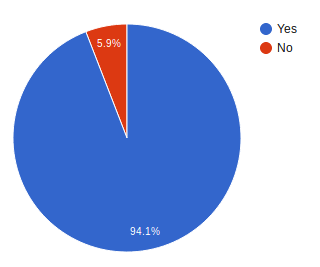
\includegraphics[scale=0.6]{Would_you_use}
\centering
\caption{Responses to whether the users would use the plugin if it was available in the IDE of their choice.}
\label{fig:wouldyouuse}
\end{figure}

As seen from the figure \ref{fig:wouldyouuse}, the majority of the users said would be interested in using the plugin (16 out of 17 responses). The majority of the justifications included similar comments to how they compared the plugin to standard issue management systems, noting its simplicity and the lack of need to switch context between the code and issue management. 

The one response that answered "No" provided the justification that in their opinion the plugin exists in the grey area between simple TODO comments and a full-suite issue management system. This is a valid statement, however, in essence this fact is exactly the purpose of the plugin and concept researched - to provide the functionality of an issue management system with the merits of quick documentation without any context switch. In addition the user noted that in order for the team members to view tickets created by others, they would firstly have to be committed which could force unnecessary commits. It is again a valid subject brought up, however, from one perspective it could also encourage the team to commit more often and incrementally as that way more electronic trace is stored.\\
\newline
\textbf{Which other functionality would you have liked the plugin to have?}
\newline
The purpose of this question was to gather feedback on which features the users thought might be missing and could be implemented in the future in order to provide a system closer to a standard issue management system but without the extra overhead of features and context switch that the standard issue management systems have.

One of the more mentioned features that the plugin could have was related to the tags of the system. Users mentioned that it would be a good quality of life improvement if the the plugin could recommend tags when a user is writing the ticket, with one user noting that a similar feature is provided by IntelliJ IDE when writing JavaDoc tags.

Another recommended improvement to the plugin was the ability to sort or filter tickets in the ticket tree by a particular attribute (priority, type etc.). This was indicated as a functional requirement as a result of requirements gathering, however, due to time restrictions and prioritising the completion of other features, this is definitely an area of improvement for future work. 

In addition, some users mentioned that the way tickets were currently displayed, there was no way to find out in which file the tickets reside unless the ticket is double clicked in the tree and they would be navigated to that file, which was deemed to be a slight inconvenience. 

\section{Summary of Evaluation}

The creation of unit tests to cover the critical sections of the application has shown that the sections covered perform as intended. User evaluation showed promising results, with a majority of users indicating the ease of use of the plugin and showing a high likelihood of using the plugin if it was available for their favorite IDEs. A good array of suggestions were given on possible improvements for the future and the issues found during evaluation either helped or might help fortify the plugin in the future. 

\chapter{Conclusion}

This chapter discusses the outcome of the project, including a summarisation of the artefacts deployed and left behind as part of documentation. In addition, possible improvements due to current shortcomings and possible additional features will be outlined as potential future work. 

\section{Project Outcome}

The developed plugin adheres to most of the functional requirements initially gathered with the exception of being able to filter and sort tickets in the task tree. The plugin was confirmed to be usable by performing user evaluation and critical sections were covered by unit tests.  

As the plugin's main purpose was to investigate the concept of microissues, a large priority was given to ensuring that the plugin would allow similar basic features as a standard issue management system and that is the case for the finished product - users are able to create and modify tickets, which are also viewable by the other team members in a group with the inclusion of being able to view a ticket's history in order to see how it has come to a particular state. 

The finished product was deployed to IntelliJ IDEA plugin repository \cite{deployed} and includes links to the GitHub page and the YouTrack issue management system that was used for documenting issues during development.   

\section{Future work}

The current plugin allows for basic features of a issue management system, however, due to the scope of the project, certain features deemed to be important had to be omitted. \\
\newline
\textbf{Sorting \& Filtering Tickets}

During the initial requirements gathering, sorting and filtering tickets by various attributes (priority, type) was considered to be a key feature alongside being able to view ticket history. However, due to time constraints, part-way through development an important choice of which feature to include in the final product had to be made. Through various considerations, ticket history was deemed to be the more important feature in demonstrating the concept of microissues. Therefore, as part of future work of the plugin, sorting and filtering of tickets would be the next logical step as in software development process it is important to prioritise actions to be taken and sorting tickets would allow the users of the plugin to either sort by priority or type of the ticket in order to view the tickets in a logical ordering. \\
\newline
\textbf{Automatic Completion of Tags}

As pointed out and suggested from a few users from the user evaluation feedback, automatic suggestion of tags when writing a ticket would be a good quality of life improvement. Most Java-centered IDEs support the suggestions for tags when writing JavaDoc comments and that is where the inspiration was most likely from.\\ 
\newline
\textbf{User-defined Tags}

In addition to using pre-defined tags, the ability to create custom attributes is a feature of some issue management systems available on the market. It is a useful feature that helps personalise a team's workflow according to what is deemed important amongst the team. The only foreseeable problem would be relating to how error prone the plugin would be and how that would tie in with sorting of the tickets if both features were implemented. \\
\newline
\textbf{Automated Building}

Initially an attempt to set up automated building was made, however, due to the particular nature of IntelliJ IDEA plugins, in particular their incompatibility with  maven, setting up a build script for the plugin turned out to be a difficult task that some plugins have achieved, although they require workarounds such as cloning the IntelliJ IDEA source code on each build. Due to the intention of the current implementation being a working prototype, not a significant priority was set on automated building due to these obstacles. However, if the plugin were to be extended and picked up by a third party in the future, configuring automated building would be extremely beneficial for testing purposes. \\
\newline
\textbf{Alternatives for Retrieving Ticket History}

The currently used approximate string matching is an experimental feature of the plugin, which is mainly used to demonstrate one of the possible ways of retrieving ticket history relating to a ticket in source code. Therefore, there might be different possible ways of doing so, which were not thought of when developing the feature. In addition, the mentioned possibility of assigning IDs in order to retrieve ticket history  could be expanded, with possibly a fully working solution devised.  

\section{Learning Outcomes \& Summary}

The development of the plugin has served as a learning experience on both personal level and gaining an insight on how issue management is perceived as part of development process, including how source code integrated issue management could be an alternative to commonplace issue management systems.

On a personal level, there was initially a lack of knowledge in both developing a plugin and the knowledge of the IntelliJ IDEA SDK. Throughout the development, new knowledge was gained of plugins' lifecycle in IntelliJ-based IDEs and the components they used. Due to the fact that a large part of the plugin used Java UI components, further reading had to be done on the various components available in order to make the plugin as intuitive as possible, as otherwise confusion might have ended up as a detrimental aspect when gathering feedback about the concept during user evaluations.  
In addition, there was valuable information gained from performing research on related plugins and research papers written on issue tracking and issue management systems, which demonstrates the importance of documentation and issue tracking for developers. It was found from the user evaluations that the concept of microissues could be a success, especially on personal projects as the majority of users noted the likelihood of using the plugin for this purpose. However, the fears of reliability of the plugin and the existing familiarity with standard issue management systems might have been the factors that prevented the users from stating with confidence that microissues could be a fully viable solution for team projects, especially consisting of a large amount of members.  

%%%%%%%%%%%%%%%%%%%%
%   BIBLIOGRAPHY   %
%%%%%%%%%%%%%%%%%%%%

\bibliographystyle{ieeetr}
\bibliography{resources/bibliography}

%%%%%%%%%%%%%%%%
%              %
%  APPENDICES  %
%              %
%%%%%%%%%%%%%%%%

\begin{appendices}
\chapter{Ethics Checklist Form}
\begin{figure}
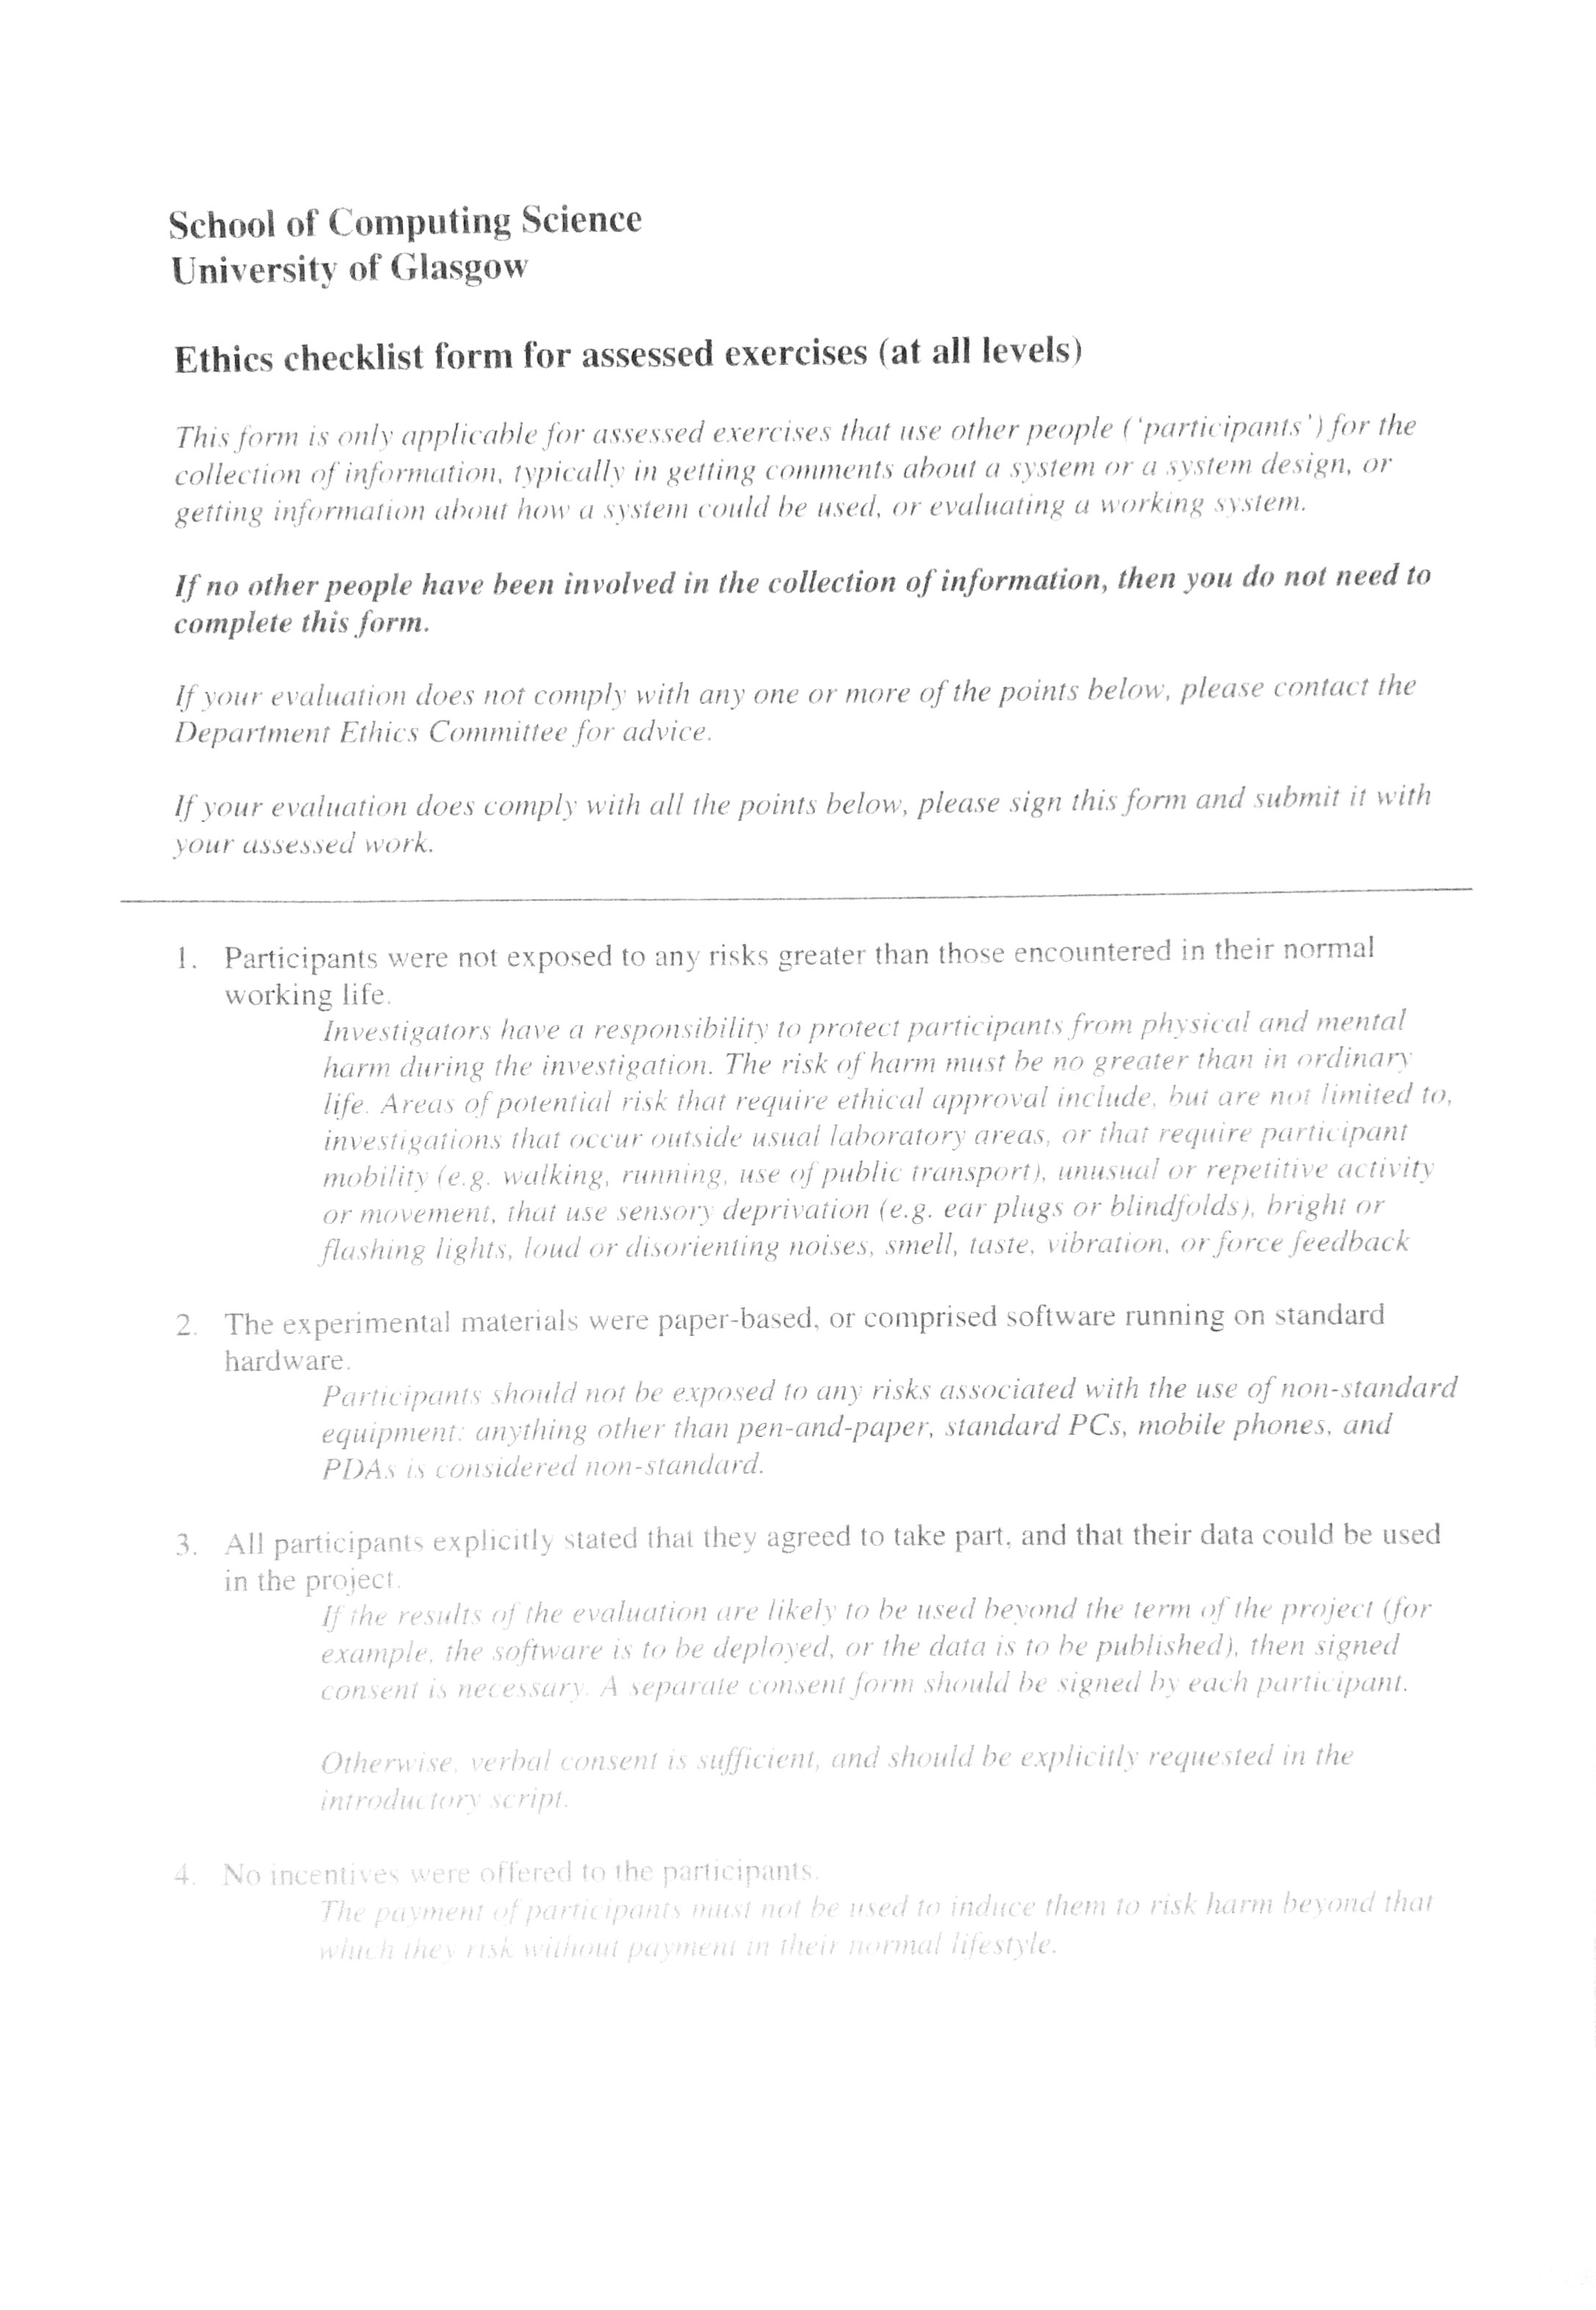
\includegraphics[scale=0.15]{Checklist_1}
\centering
\caption{The first page of the ethics checklist form}
\label{fig:Checklist1}
\end{figure}

\begin{figure}
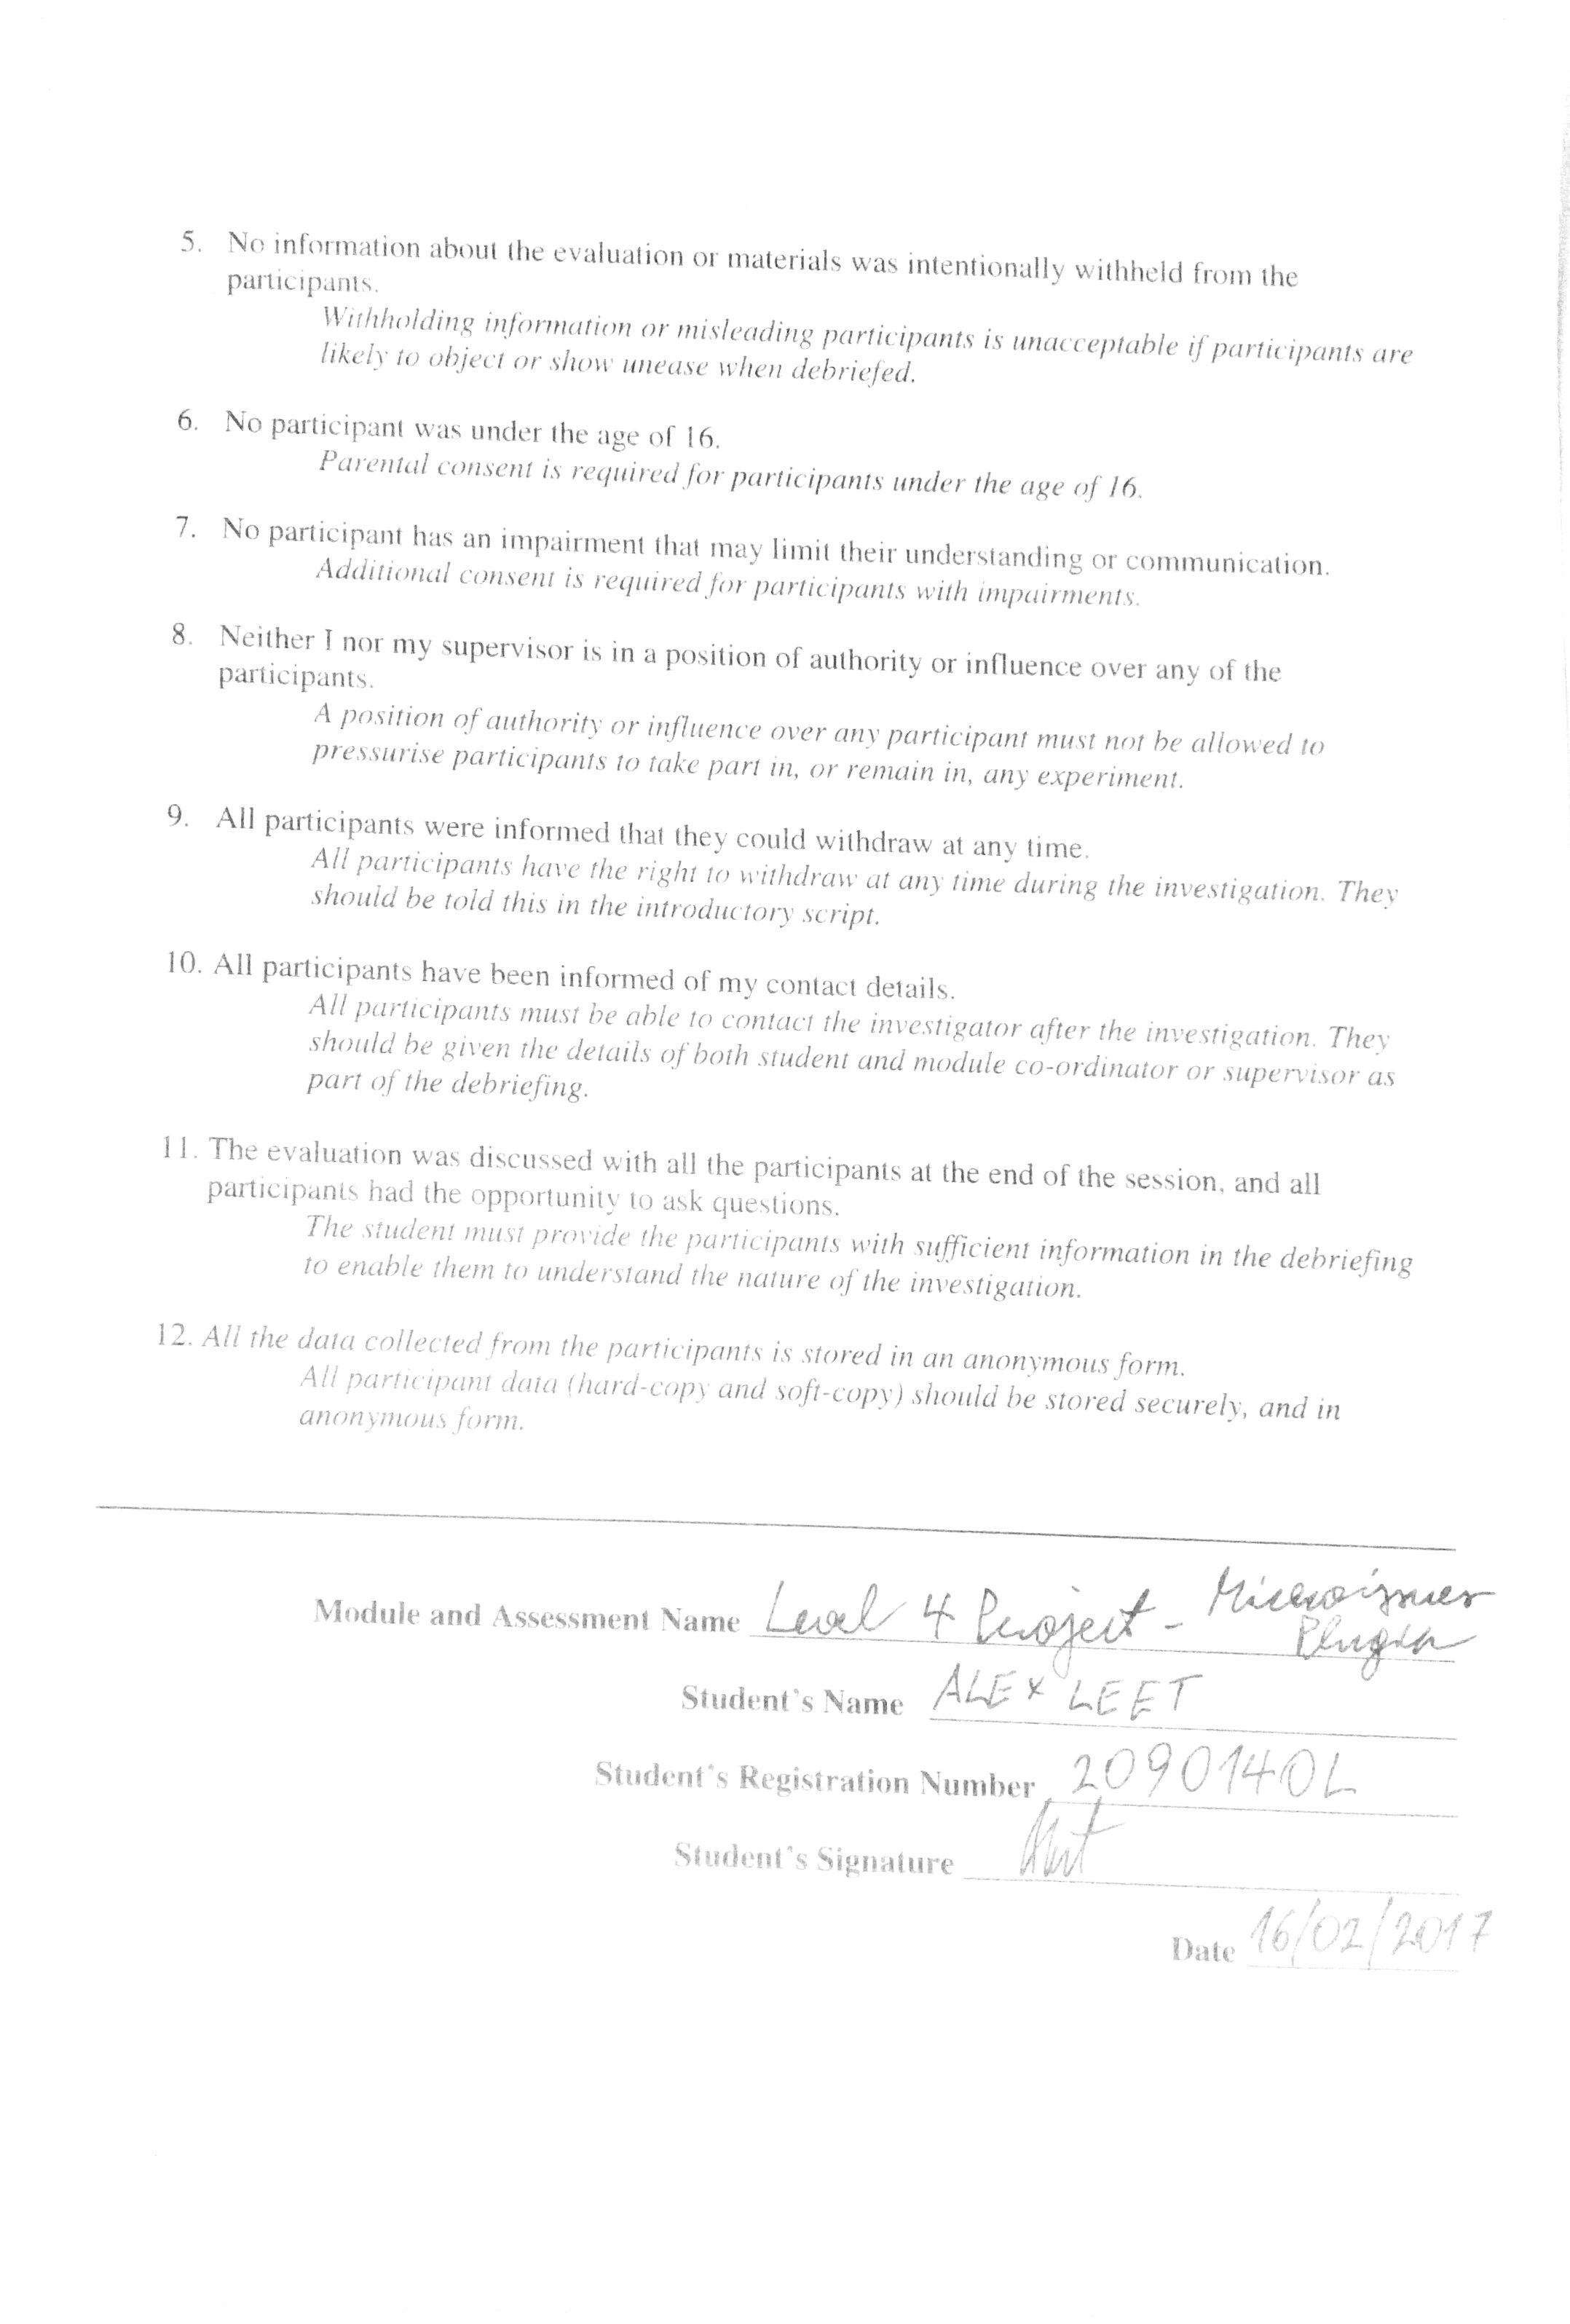
\includegraphics[scale=0.15]{Checklist_2}
\centering
\caption{The second page of the ethics checklist form with filled in details.}
\label{fig:Survey_1}
\end{figure}

\chapter{Survey Questions}

\begin{figure}
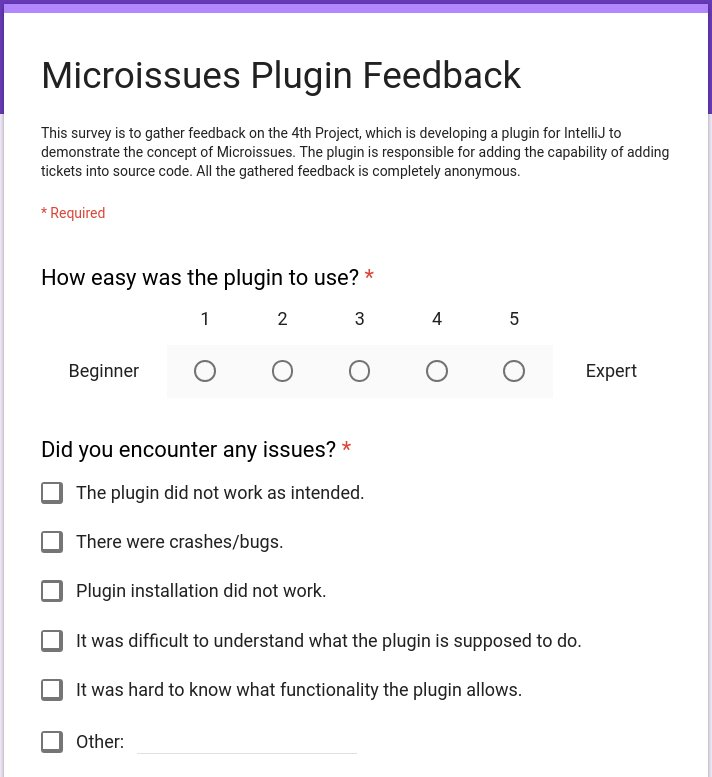
\includegraphics[scale=0.5]{Survey_1}
\centering
\caption{The first set of questions of the survey.}
\label{fig:survey1}
\end{figure}

\begin{figure}
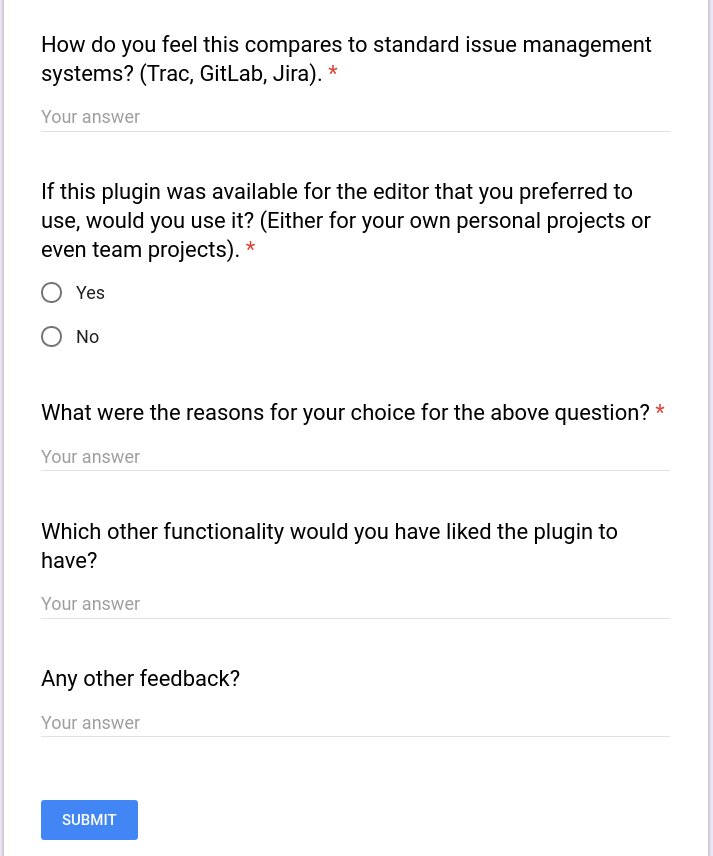
\includegraphics[scale=0.5]{Survey_2}
\centering
\caption{The second set of questions of the survey.}
\label{fig:survey2}
\end{figure}

\chapter{Qualitative Data from the Survey Feedback}

\begin{figure}
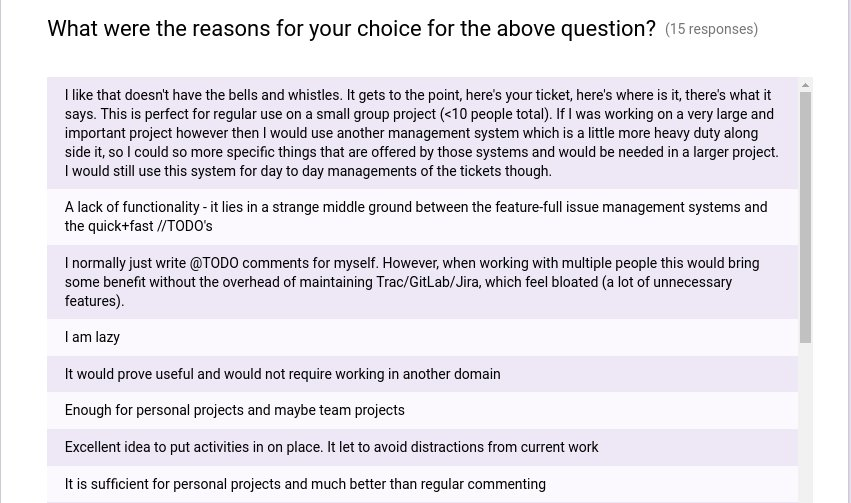
\includegraphics[scale=0.5]{Reasons_for_choosing}
\centering
\caption{The reasons justifying why the users would use the plugin Part 1.}
\label{fig:reason1}
\end{figure}

\begin{figure}
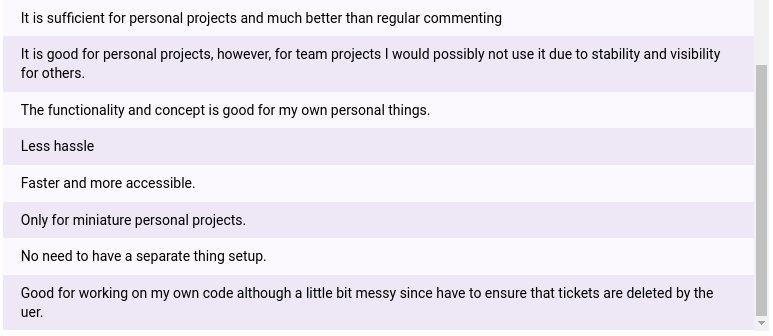
\includegraphics[scale=0.5]{Reasons_for_choosing2}
\centering
\caption{The reasons justifying why the users would use the plugin Part 2.}
\label{fig:reason2}
\end{figure}

\begin{figure}
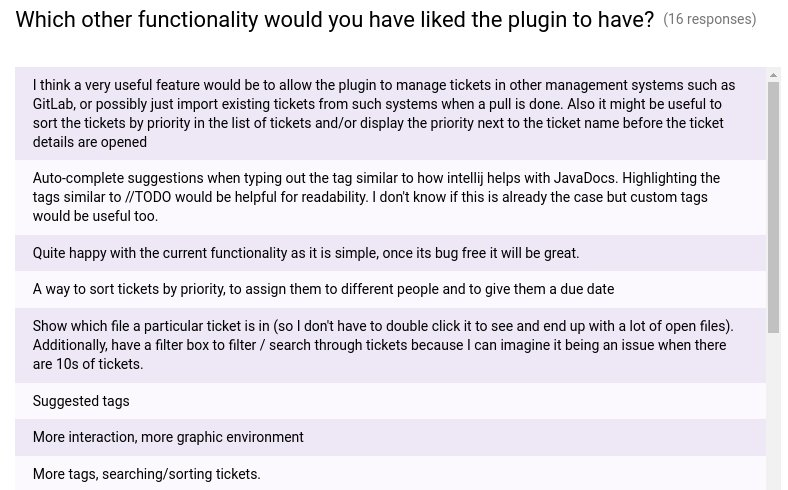
\includegraphics[scale=0.5]{Other_function}
\centering
\caption{Additional features the users can envisage Part 1.}
\label{fig:func1}
\end{figure}

\begin{figure}
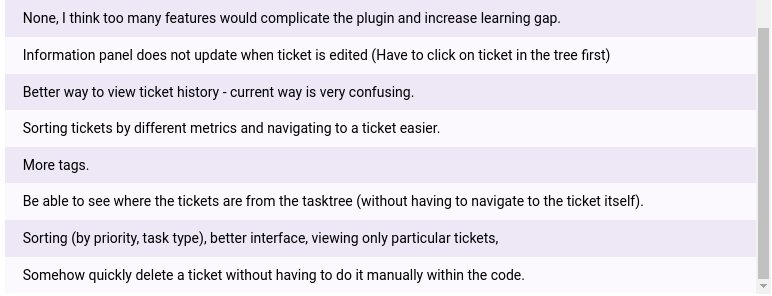
\includegraphics[scale=0.5]{Other_function2}
\centering
\caption{Additional features the users can envisage Part 2.}
\label{fig:func1}
\end{figure}


\begin{figure}
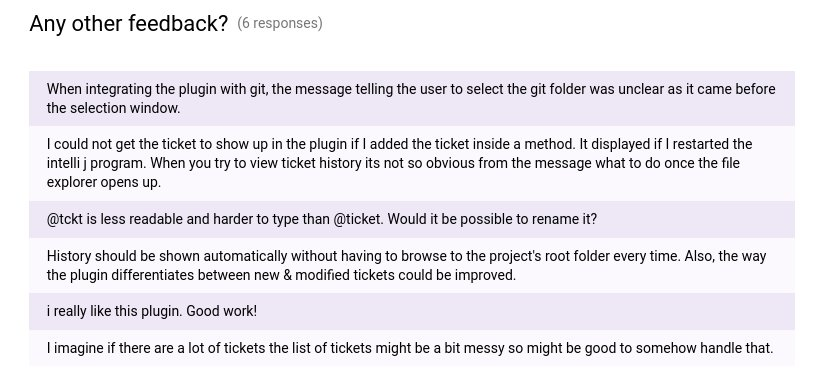
\includegraphics[scale=0.5]{Any_other_feedback}
\centering
\caption{Any additional feedback the user might have.}
\label{fig:anyother}
\end{figure}
\end{appendices}



\end{document}
